\documentclass[a4paper,12pt]{report}

\usepackage{amsfonts}
\usepackage{amsmath}
\usepackage{amsthm}
\usepackage{amssymb}
\usepackage{graphicx}
\usepackage{dcolumn}
\usepackage{fullpage}
\usepackage{enumerate}
\usepackage{rotating}
\usepackage{setspace}
\usepackage{bm}
\doublespacing

\newcommand{\ve}[1]{\ensuremath{\mathbf{#1}}}
\newcommand{\vbeta}{\boldsymbol{\beta}}
\newcommand{\R}{\mathbb{R}}

\usepackage[american]{babel}
\usepackage{csquotes}
\usepackage[style=apa,natbib=true,backend=biber]{biblatex}
\DeclareLanguageMapping{american}{american-apa}
\addbibresource{Polarization.bib}

\newtheorem{assumption}{Assumption}

\newcommand{\bmu}{\boldsymbol{\mu}}%

\usepackage[colorlinks,allcolors=blue]{hyperref}
\hypersetup{%
    pdftitle={Tasks, occupations, and the polarization hypothesis},%
    pdfauthor={Alex Cooper},%
    pdfsubject={An analysis of one determinant of inequality in Australia.},%
    pdfkeywords={labor, polarization, routinization, SBTC, inequality},%
}
\ExecuteBibliographyOptions{doi=false}
\newbibmacro{string+doi}[1]{%
  \iffieldundef{doi}{#1}{\href{http://dx.doi.org/\thefield{doi}}{#1}}}
\DeclareFieldFormat{title}{\usebibmacro{string+doi}{\mkbibemph{#1}}}
\DeclareFieldFormat[article]{title}{\usebibmacro{string+doi}{\mkbibquote{#1}}}

\numberwithin{equation}{chapter}

\begin{document}
% yeah yeah yeah I know
% plenty of time for this
\title{Jobs, Tasks, and Technology}
\author{Alex Cooper}
\maketitle

\begin{abstract}
Could technology be responsible for part of the rise in income inequality over the past 30 years? This research is motivated by the fact that, while technology can make workers more productive, it can also render other workers unneccessary by automating some tasks. By changing demand patterns for different kinds of labor, it is possible that technology is responsible for an increase in the demand and wage of certain types of work, and a reduction in the wage and number of others. Research from the United States and Europe suggests that technological change has indeed caused such a `polarization' of the wage distribution.

In this thesis, we assess the evidence for polarization in Australia. We first consider the standard model of skill-biased technical change, and show that it only poorly fits the observed data. We link the wage share of middle-skilled occupations to investment in electronic and electrical capital goods, and also demonstrate a relationship between qualitative properties of certain jobs, and changes in the wage distribution. We find that jobs of the kind most likely to be impacted by technology, so-called `routine' jobs, have suffered the greatest decline in income over the past 30 years, and that the penalty associated with routine work is concentrated in upper wage quantiles. Finally, we find a large change in the value of occupations involving managerial tasks, an effect that may or may not be associated with technical change.
\end{abstract}

\tableofcontents{}

\chapter{Introduction}

%%% Local Variables: 
%%% mode: latex
%%% TeX-master: "thesis"
%%% End: 

\chapter{Skill-biased technical change}

We begin our exploration of income inequality with an analysis of labor-augmenting technology.

\section{Related Literature}

Much of the economic literature views production through the lens of the neoclassical production function, which simply `converts' inputs of capital and labor into an output good. Most formulations of the production function include a `productivity' parameter, that governs the rate at which factors of production are converted into outputs. Solow's (\citeyear{Solow1957}) well-known functional form, $F(K,L,t)=A(t)f(K,L)$, included measures for capital ($K$) and labor ($L$) inputs, but also allowed `technology' ($A(t)$) to vary over time. He deliberately left the definition of technology vague, to simply mean any change in the rate of production: ``all sorts of things will appear as technical change'' \citep[p.312]{Solow1957}.

By inverting his production function and assuming a functional form for $f$, Solow was able to impute values for $A(t)$ as the `residual' output not explained by the neoclassical production function. In his 1957 paper, Solow employed US national accounting statistics for real GDP, capital and labor. Between 1909 and 1949, Solow's estimates for total factor productivity increased more or less monotonically, and by 1949 $A$ had grown to double its initial value. Taken together with Solow's (\citeyear{Solow1956}) model of long-run growth, one important use for Solow's contribution was to spur the field of growth accounting. This approach to studying income spawned a large empirical literature studying the causes of economic growth and development. Today, the neoclassical approach remains an important class of models in the study of the patterns of international income and growth. A prominent example is \citet{Mankiw1992}, which shows that the Solow model, augmented for a measure of human capital, explains cross-country variation in incomes very well indeed.

In the 1980s, empirical evidence from the United States suggested that the rental rate of skilled workers began to grow considerably faster than that of unskilled workers. Until then, wage growth differentials between different skill and educational groups had remained more or less stable. Solow's simple but elegant model, which makes no distinction between different kinds of workers, does not provide any insight into this trend. A number of modifications to the theory were advanced. 

One set of explanations pointed to the changing nature of labor market institutions. \citet{Freeman1994}, for example, suggested that the about 50 per cent of the increase in the `white collar' premium paid to U.S. men could be explained by the decline in the unionization rate. It is widely understood that union bargaining activities result in a narrowing of wage dispersion between unionized workers. He argued that a decrease in the union rate resulted in a loss of worker bargaining power, and thus a decrease in wages. But since unions tend to cover mainly `blue-collar' occupations, then this trend should result in a widening gap between blue- and white-collar work. Yet other explanations for the growing premium paid to skilled workers include sociological factors, such as changes in norms associated with worker pay, \citet{Mitchell1989}. Alternatively, the decline in the density of union workers may simply reflect broader economic trends: changes in the nature and distribution of production activity, for instance.

Such an explanation was advanced by \citet{Murphy1992}, who appeals to changes in the demand structure of US labor as a consequence of trade and competition with overseas producers. The patterns of U.S. trade shifted over the 1980s to trade deficits, favoring the manufacture of goods in low-cost countries, instead of with domestic, high-cost workers. The authors study the relationship between wage rates for white males between 1963 and 1979, and macroeconomic measures of output and wages both in the U.S. and overseas, concluding that changing patterns of trade go a long way to explain changes in the wage structure.

During this debate, some authors argued that technological progress might have softened demand for certain kinds of physical labor. Using logitudinal data gathered from census files, \citet{Davis1991} argue that, though capital investment in automated equipment and machinery, the manufacturing sector  replaced labor-intensive jobs with plant capital. Under this explanation, growing wage differentials between college-educated workers and high school graduates is a result of changes in the demand for labor, as the demand for non-manual work expands, and the demand for manual labor softens. \citet{Krueger1993} expands on this argument, and using microdata on individual workers, finds a premium associated with those occupations that involve computer use.\footnote{For a rather cynical refutation of Krueger's position, see \citet{DiNardo1997}, who show that an effect of a similar magnitude is associated with occupations that use pencils.}

However, the predominant explanation that came to be accepted in the literature is that new technologies, emerging over the post-war era, are complementary to skilled work. \citet{Tinbergen1974,Tinbergen1975} developed a model of the labor market where different kinds of labor were factors in production. Since the time of Adam Smith, it has been well known that the productivity of modern production processes, at any scale, depends crucially on the specialization of labor into a number of different jobs. In Adam Smith's famous study of a pin factory, Smith observed somewhere between a 240-- and 4800--factor increase because of complementarities between different, specialized jobs \citet[I.3]{Smith1910}. Tinbergen recognized that it would be unwieldy to attempt to model every of job using a production function, as the dimensionality of the model would quickly explode. However, armed with the observation that many properties of jobs are highly correlated, he proposed that a good characterization of the labour market can be made by singling out just one or two properties of different jobs. One particularly relevant property of jobs is the degree of {\em schooling} an individual has received. \citet{Tinbergen1974} modeled `graduate' and `unskilled' workers as imperfect substitutes in production, so that firms would seek to employ some number of both types of workers. 

Tinbergen identified two implications of his model. First, since the higher-productivity `graduate' workers were scarce relative to the supply of unskilled workers, graduates would be able to charge employers `scarcity rents,' as well as additional rents for their individual productivity. In the medium run, the availability of these rents would initiate a `race' for investment in education, as unskilled workers seek to enter education in order to access these rents.

Tinbergen's model was further developed by \citet{Katz1992} and others, and brought to bear on the empirical regularity of rising educational returns in the United States and elsewhere, beginning in the 1980s. In their model, they suggest that new workplace technologies disproportionately complement highly-skilled technical and managerial jobs, relative to low-skilled manual and service jobs. Under this explanation, the premium paid to high-skilled labor increases for two reasons: first, since high-skilled workers become relatively more productive, wages to high-skilled occupations are higher at the margin. There is also evidence that, in the United States at least, an increase in the demand for skilled labor, relative to its supply, has resulted in higher wages for skilled occupations. In the jargon, such technologies are said to exhibit \emph{skill bias} \citep{Autor2006}. 

\section{The `Canonical Model' of SBTC}

One formulation of the SBTC model, dubbed the `canonical model' by \citet{Acemoglu2011}, gained wide acceptance in the literature, and was deployed by a large number of authors analyzing skill-biased technology \citep[e.g.]{Katz1992,Goldin2007}. % etc
Before discussing the empirical evidence for SBTC, we will briefly outline the main features and implications of this model, following the notation employed by \citet{Acemoglu2011}

Consider a competitive economy with two different, imperfectly substitutable types of labor: high-skilled and low-skilled. Workers are heterogeneous, with different levels of efficiency within each skill group. Let the total supply of high-skilled labor be $H$, and the total supply of low-skilled labor be $L$, and both types are paid the same wage, respectively $w_h$ and $w_\ell$. Production in this economy is governed by a CES aggregate production function, with elasticity of substitution $\sigma$, where $\sigma>1$:
\begin{equation}  \label{eq:prod}
Y = \left[
  \left(A_LL \right)^\frac{\sigma-1}{\sigma}
  +
  \left(A_HH \right)^\frac{\sigma-1}{\sigma}
  \right]^\frac{1}{\sigma-1}.
\end{equation}

For our purposes, we are interested in two claims about relative wages made by this model: first, that technological change or a generalized shift from low-skilled to high-skilled work should never cause low-skilled wages to decrease, and second, that technological change should result in a monotonic increase in wage across the skill spectrum. To see this, we will first derive the expressions for the equilibrium wage for each type of labor. Since the economy is competitive, unique equilibrium wages for both both high- and low-skilled workers are given by their respective marginal products. Wages can therefore be found by differentiating \eqref{eq:prod} with respect to labor supply:
\begin{align}
w_h &= \frac{\partial Y}{\partial H} 
     = A_H^\frac{\sigma-1}{\sigma}\left(
              A_L^{\frac{\sigma-1}{\sigma}} (H/L)^{-\frac{\sigma-1}{\sigma}} + A_H^{\frac{\sigma-1}{\sigma}}
        \right)^{\frac{1}{\sigma - 1}} \label{eq:wh} \\
w_l &= \frac{\partial Y}{\partial H} 
     = A_L^\frac{\sigma-1}{\sigma}\left(
              A_L^{\frac{\sigma-1}{\sigma}} + A_H^{\frac{\sigma-1}{\sigma}}(H/L)^{\frac{\sigma-1}{\sigma}}
        \right)^{\frac{1}{\sigma - 1}} \label{eq:wl}
\end{align}
The first claim follows from differentiating these wage equations. First, notice in \eqref{eq:wl} that $\partial w_L/\partial A_H \geq 0$. This means that, in this model, an increase in technology for high-skilled workers does not reduce the wage for low-skilled workers. Technological progress should in fact result in positive wage improvements for both high- and low-skilled workers. 

Next, notice that $\partial w_l/\partial(H/L)>0$. An increase in the relative supply of high-skilled workers, $H/L$, should therefore not decrease the wage of low-skilled workers. Rather, as high-skilled work becomes more productive and the ratio of skilled to unskilled workers increases, the demand for low-skilled work simultaneously increases. 

Second, consider the ratio between high- and low-skilled labor, $\omega=w_h/w_l$ (for convenience, we will consider the log ratio.) It is straightforward to show that this ratio depends on the state of technology and labor inputs:
\begin{equation}\label{eq:omega}
\log \omega = \frac{\sigma-1}{\sigma}\log\left(\frac{A_H}{A_L}\right) - \frac{1}{\sigma}\log\left(\frac{H}{L}\right).
\end{equation}
This equation illustrates the two countervailing forces of Tinbergen's (1974) `race' for education that govern the magnitude of the skill premium. Holding the labor supply ratio constant, and recalling our assumption that $\sigma >1$, an increase in skill-biased technology $A_H/A_L$ results in a larger $\log\omega$. On the other hand, holding technology constant, an increase in the proportion of workers providing high-skilled labor should decrease the log skill premium.\footnote{Formally, $\partial \log\omega / \partial(A_H/A_L) > 0$, and 
$\partial \log\omega / \partial(H/L) < 0$.} In this model, a rising skill premium occurs when the first term of \eqref{eq:omega}  dominates the second.

To review, the SBTC model claims that unless there is technical regress, wages for all skill types will always increase, and never decrease (wages should follow a monotonic path.) Second, in the presence of an increasing proportion of workers conducting skilled work, the model is consistent with either a rising or a falling log skill premium.

\section{Empirical Evidence for SBTC}

%Between 1960 and the 1980s, the pattern identified by Solow continued: as the economy grew, income accruing to workers steadily increased. In the United States, during this period the composition of the workforce changed as women entered the workforce, and the educational attainment of women and blacks increased. Likewise in Australia, 

Starting in the 1980s, in the United States a divergence between the rental rates of skilled an unskilled labor began to emerge. \citet{Acemoglu2011} report that the `skill premium' paid to college-educated workers remained relatively steady between 1964 and 1980, oscillating in the range of between 48 and 58 per cent, holding other factors constant. However, from 1980, this premium increased steadily 


We will take as a point of departure the standard model for analyzing skill-based technical change (SBTC). This model, dubbed the `canonical' model by \citet{Acemoglu2011} and which has sparked a voluminous literature, has enjoyed considerable empirical success explaining rising wages for high-skill managerial and professional jobs in the United States and Europe \citep{Katz1992}. Since the canonical model includes \emph{factor-augmenting} capital, it predicts a uniform skill upgrading of the work force at all education levels \citep{Levy2003}. Skill upgrading has been confirmed by a number of authors, both in Australia \citep{Esposto2012, Wooden2000, Cully1999} and overseas \citep{Autor2008}. 

\section{Data}

To bring the SBTC model to the data, we employ the Survey of Income and Housing, a hierarchical clustered household survey conducted by the ABS every 2-3 years since 1995, and also for the fiscal years 1985-6 and 1981-2. The survey provides detailed  information about respondents' labor and non-labor income sources, as well as data on age, educational attainment, hours worked and industry and occupation. For the surveys conducted between 2000 and 2010, as well as the 1981-2 survey, the data include detailed occupational data, which will become important later. The other surveys include occupation only at the one-digit level. We obtain survey micro-data as confidentialized unit record files (CURFs).

To facilitate inter-temporal comparisons, we must eliminate effects which arise as a result of mechanical, demographic shifts. Between 1982 and 2010, the number of women in the work force has increased dramatically, and the same period has seen an evolution of the educational and age composition of the work force, and the rate of casual and part-time employment has increased. Following \citet{Acemoglu2011}, we therefore include only full-time workers for whom labor forms the primary source of income. We further composition-adjust each survey to match 2010 demographics by linearly scaling the survey selection weights for each age group/sex/educational group cell. All computations in this study treat these adjusted weights as inverse selection probabilities.

\begin{figure}
  \centering
  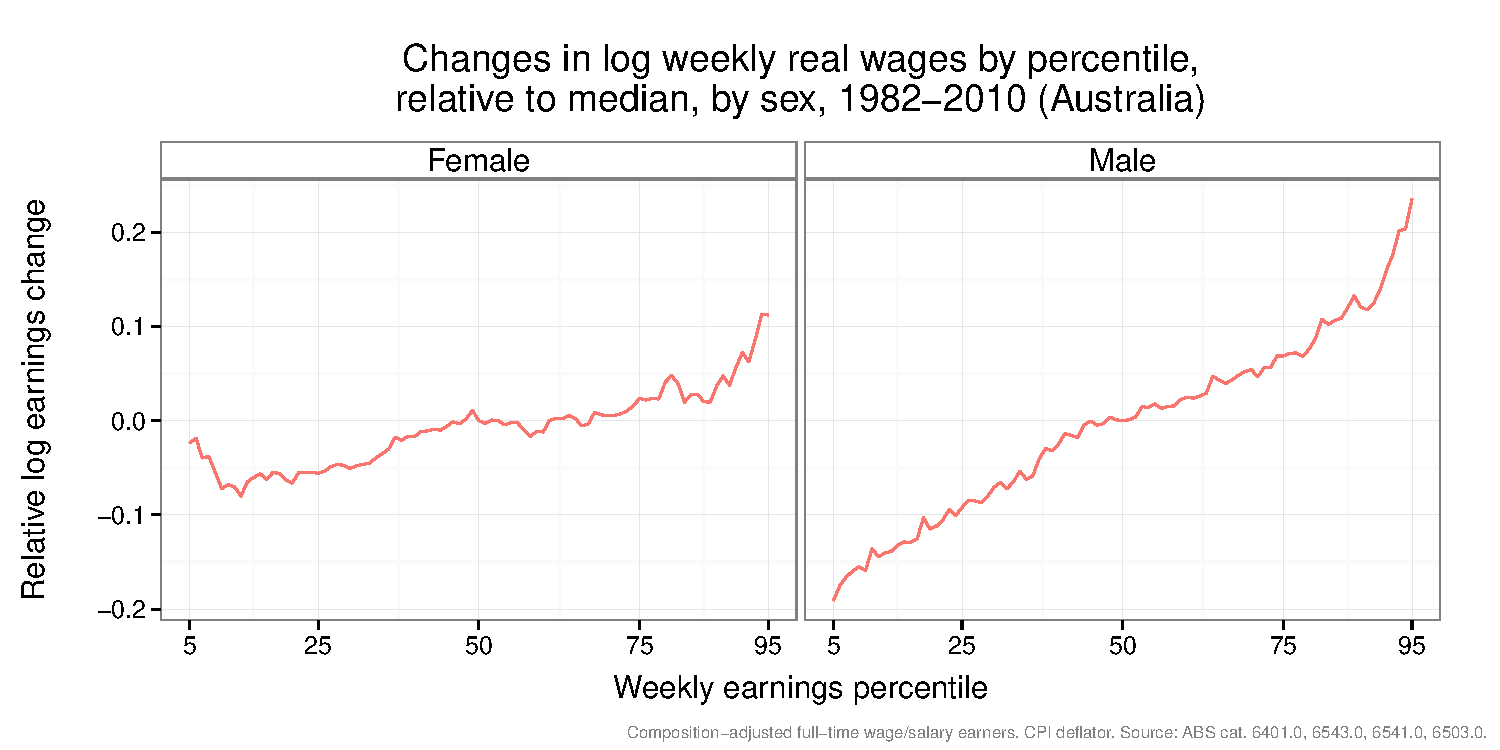
\includegraphics[width=\textwidth]{../figure/quantile_mf.pdf}
  \caption{Change in weekly wage by percentile, 1981-2010, Males and Females. Full-time workers whose main sources of income are wages and salaries are shown. Notice that real wage growth has been non-monotone for males in lower percentiles. Source: Survey of Income and Housing.}
  \label{fig:banana}
\end{figure}

\section{Results}

If SBTC explained the widening of the income distribution, we would expect to observe the premium accruing to `skilled' labor increasing with time. Figure~\ref{fig:banana} shows the composition-adjusted changes in log real wage by percentile, for males and females, between 1981-82 and 2009-10. If the 1981-82 income percentile can be considered a proxy for skill, then it is apparent that, over this period, wages more grew for high-skill individuals much faster than for low-skill individuals. It would therefore be expected that the premium accruing to higher educational attainment would show a similar trend.

In the United States, at least, the wage premium earned by tertiary-educated labor fell in the 1970s, but has risen each decade since then \citep{Acemoglu2011}. \citet{Katz1992} employs a similar empirical model which explains the rise of the skill premium in the United States in the post-war era. In Australia, however, a corresponding growth in the premium for tertiary qualifications has not been observed. Table~\ref{tbl:wagepremium} shows the log skill premium for Australia and the United States between 1982 and 2008. Rather than any fundamental differences in the nature of the demand for skills, \citet{Coelli2009} attributes this difference in Australian workers to differences in the nature of Australian educational qualifications. In Australia, University degrees are available to a wider range of candidates and for a wider range of disciplines than those who would traditionally have undertaken university studies in the United States. As a result, tertiary educational attainment may be a poor proxy for `skilled' work in Australia.
\begin{table}
  \centering
  \begin{tabular}{lcc}
  \hline
           & \multicolumn{2}{c}{\bf Log Skill Premium} \\
\hline
{\bf Year} &	{\bf United States} & {\bf Australia} \\
{\bf 1982} &	0.42 &	0.42 \\
{\bf 1995} &	0.59 &	0.36 \\
{\bf 2003} &	0.64 &	0.37 \\
{\bf 2008} &	0.68 &	0.34 \\ \hline
\end{tabular}
  \caption{University/non-university log wage premium, Australia and the United States. The figures show the difference between the mean log weekly income for workers who have attained a bachelor degree or higher, and the mean weekly income of other workers. Only full-time workers whose main sources of income are wages and salaries are included, and survey data have been composition adjusted for sex, age group, (and for the United States, race). Source: for Australia, ABS Survey of Income and Housing, and for the United States, \citet{Acemoglu2011}.}
  \label{tbl:wagepremium}
\end{table}

The SBTC model also claims that, even if technology exhibits skill bias, wages for all skill groups should increase monotonically. Figure~\ref{fig:changetime} plots the cumulative change over time for three wage percentiles, the 5th, 95th, and the median. Over the period 1981-82 to 2009-10, although wages at the top percentiles increased steadily, the same is not true for the lower percentiles. Indeed, for all of the 1990s and much of the 2000s, cumulative real income growth from 1981-82 was negative for many workers.
\begin{figure}
  \centering
  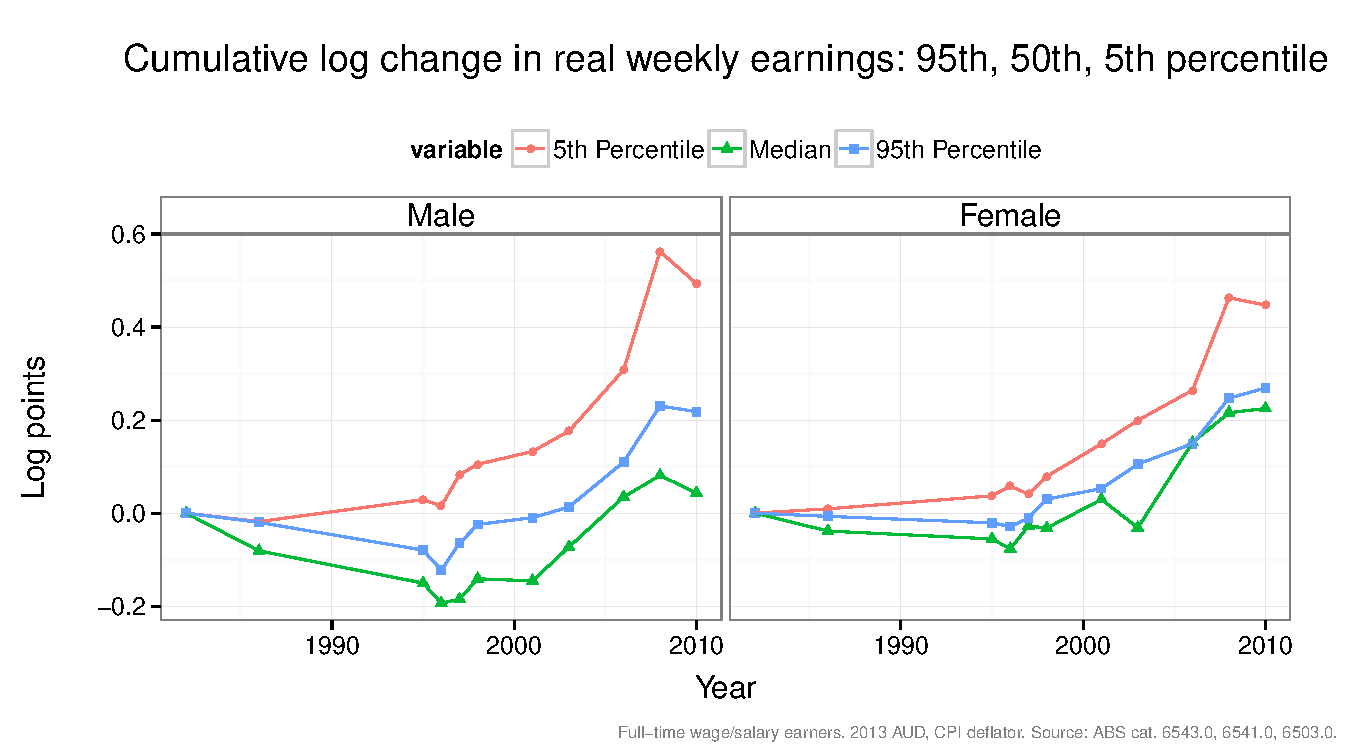
\includegraphics[width=\textwidth]{../figure/wage_change_time.pdf}
  \caption{Cumulative log change in real weekly earnings, 5th, 50th and 95th percentiles, 1982-2010. Full-time workers whose main sources of income are wages and salaries are shown. Notice that real wage growth has been non-monotone for males in lower percentiles. Source: Survey of Income and Housing.}
  \label{fig:changetime}
\end{figure}

That the income distribution is widening, but the skill premium is {\em not} driving the change, suggests one of at least two interpretations. We have already discussed the fact that educational attainment may be a poor indicator of skill for the Australian labor market. A second, more nuanced explanation was given by \citet{Levy2003}. Technological change may not be complementary to all types of labor; it may replace many types of labor entirely.





%%% Local Variables: 
%%% mode: latex
%%% TeX-master: "thesis"
%%% End: 

\chapter{Empirical Literature}\label{ch:3}

In this chapter, we review empirical evidence for the models discussed in Chapter~\ref{ch:2}. To some extent, the distinction between the theoretical and empirical literture is artificial: models of wage differentials and technology are difficult to separate from the empirical regularities that they describe. Nonetheless, in this section, we discuss four broad classes of studies.

First, we briefly discuss results from demographic studies of the work force. These `model-free' studies are important because they provide the empirical regularities that models are intended to explain. Second, we look at estimates of skill changes, based on classification schemes and other measures. Third, we discuss estimates of neoclassical models of the labor force, in which model parameters are calibrated to mean values derived from survey and aggregate data. Finally, we review some examples of decomposition-type studies, in which non-parameteric and semi-parametric evidence for wage-setting models are drawn from wage distribution.

There is a large body of evidence for upskilling and polarization in foreign labor markets; indeed this evidence prompted much of the research into skill-biased technical change. We touch briefly on these studies, but where possible, our focus here is on Australian research. Somewhat surprisingly, since one of the key explanations for SBTC includes globalization and the worldwide proliferation of new technology, the evidence for SBTC in Australia is does not exactly match the US and European experience. However, many studies have confirmed a growing demand for skilled labor, as well as an associated growth in its supply.

\section{Direct Measures of SBTC}\label{sec:direct}

One way to determine whether technology is skill-biased is to directly analyze the properties and wage distributions of jobs that use new technologies. One advantage of this type of study, is the absence of an economic model---so the results are less susceptible to specification biases. To support the claim of SBTC, there are two claims that we want to see verified from sample surveys: first, that technology adoption is growing, and that the nature of work changes as a result (existence of technical change). Second, we expect to see that this technology impacts primarily on those with high skills (existence of skill bias).

Qualitiative research on the nature of computerization strongly supports the claim that technology dramatically changes workplaces. Evidence from the US Current Population Survey confirms that, during the 1980s and 1990s, there was indeed an increased incidence of computer use in the workplace. Between 1984 and 1997, the data show that the the proportion of individuals using computers at work increased from 24\% to 51\% \cite{Friedberg2003}. Furthermore, evidence from the 1990s shows that the introduction of new technology results in a substantial rearranging of work patterns. \citet{Levy1996} studied the application of new technology to automate tasks in a financial services firm. He found that, although technology process simplified many of the processes, those that were not automated became more complicated. Similarly, \citet{Autor2002} studied the introduction of digital check imaging in a large bank, and found that, while many `routine' tasks were easily automated, substantial changes occurred in those tasks that could not be performed by machiens. \citet{Bresnahan2002} offers evidence that the introduction of computers into workplaces often incurs significant adjustment costs, including re-training, re-organization, and so on.

A limited number of surveys have been conducted in Australia. \citet{Borland2004} employs a cross-sectional survey of Australian workers, the 1993 ABS Training and Education Experience Survey (TEES). This survey included detail of workers' skills and depth of computer knowledge, as well as interval-censored earnings information. Using interval regression techniques, Borland regressed a number of human capital, experience and job characteristic variables against income, worker characteristics and proxies for skills, as well as a categorical variable concerning computer use and experience. 

Without controls, the return to computer use in 1993 is estimated at 18 per cent of earnings; however, once controls are included, this effect reduces to about 8 per cent. One problem with this type of study is that, since computer use is associated with high-skilled work, individuals' unobserved ability is likely to be correlated with computer use. Despite the inclusion of proxies for individual skill and ability, this means that the return to computer use cannot be exactly identified. Nonetheless, this study does strongly suggest the presence of a skill premium in the Australian labor market.

\section{The `College Premium'}

Beginning in the 1980s, a divergence between the rental rates of skilled an unskilled labor began to emerge in the US. \citet{Acemoglu2011} report that the `skill premium' paid to college-educated workers remained relatively steady between 1964 and 1980, oscillating in the range of between 48 and 58 per cent, if other factors are held constant constant. However, from 1980, this premium increased steadily, far outpacing the growth rates of other types of labor, dramatically increasing wage inequality between income groups. This trend was documented using CPS microdata by \citet{Karoly1992} and \citet{Katz1989}, among others, using reported educational attainment to identify individuals into groups.\footnote{The US experience was not universal: \citet{Katz1989} found, for example, that Japanese wage differentials had not followed the same pattern.} These studies also identified an intensification of the proportion of workers in the US with tertiary qualifications. To some extent, there were factors unrelated to the work force that could be explain this jump in educational attainment: in the 1970s, students who continued college study were exempt from service in Vietname, and returning veterans were granted scholarships via the G.I. bill \citet{Acemoglu2011}. Nonetheless, the two labor market trends emerging from this literature were a continual `up-skilling' of the workforce since the 1980s, and a steady increase in the `college premium', the average premium paid to workers who had attained college degrees or higher.

\subsection{Upskilling in Australia}\label{sec:upskillingau}

`Skills' in the Australian labor market have been identified in empirical studies using (at least) two methods. The first, as with the US studies outlined above, is to use educational attainment. The second, is to use occupational group as a proxy for skill.

In sample surveys, occupations must be coded according to some consistent scheme in order to be comparable across the sample survyed, and also across time periods. The occupational classification schemes used in Australia, such as the ASCO \citep{Castles1986}, and the ANZSCO \citep{Trewin2006}, typically include a `skill level' ranking for each coded occupation. The ASCO II, defines skill level as `a function of the range and complexity of the set of tasks involved' \citep[p.14]{Castles1986}, and is a combination of the level of education and experience required for classified occupations. The use of these skill metrics have been criticized, but they do provide useful categories for analysis of the skill distribution can be performed.\footnote{\citet{Cully1999} argues their use originates from the need to place employees in a social class, rather than analyze the skill intensity of the work. However, it is not clear that these skill levels are any worse than the use of educational attainment as a skill proxy.}

\citet{Cully1999} divides employment data into five broad skill groups, and analyzes changes in the number of jobs at each category between 1986 and 1997.\footnote{These groups are aggregations of the top-level groupings given in the ASCO, and are the same was those later used by \citet{Wooden2000} and \citet{Esposto2012}. The skill groupings are, (1) managers/professionals, (2) associate professionals, (3) skilled vocations, (4) intermediate skills, (5) elementary skills.} He finds that, over this period, there was growth in the high- and low-skilled jobs, but that the number of jobs in the middle categories was stagnant or declined, lending some support to the polarization hypothesis. However, in line with international evidence, the dominant pattern in the data is growth in high-skilled jobs, or `up-skilling.' A similar conclusion is reached by \cite{Wooden2000}, who expands Cully's methodology to also consider growth in terms of hours worked.

A more recent analysis of the skills distribution was undertaken by \citet{Esposto2012}, who adopts the aggregation approach taken by \citet{Cully1999}, but using a longer sample, and using Census data, between 1971 and 2006. By recombining the 1971 census data, which was coded using an obsolete coding scheme, to suit the ASCO II classification, Esposto is able to create a comparable series of the levels of occupations over this 35-year period. Novel in Esposto's analysis is a breakdown of full-time and part-time work.

Esposto finds that, between 1971 and 2006, the skill intensity of the Australian labor market increased, as measured by a greater proportion of the work force employed in high-skill occupations. The greatest growth was observed in the top category, professionals and managers (115.5 per cent), and the two lowest skill categories, intermediate and elementary skills, also grew (54.5 and 22.5 per cent, respectively). The middle category, `skilled vocations' shrank by 7.4\%, suggesting job polarization. Furthermore, Esposto disaggregated part-time and full-time jobs, and found that full-time jobs predominantly experienced upskilling, whereas part-time and casual jobs experienced down-skilling, especially for males.

\subsection{A `Uni Premium' in Australia?}

Somewhat surprisingly, college premia are not readily apparent in the Australian data. \citet{Barnes2002} analyze household survey data, and use educational attainment as a proxy for skill. They find that, over the 1980s and 1990s, growth in the demand for high-skilled far outpaced that of low-skilled workers. In the 1980s, the demand for skilled employment grew at a rate of 4.7 per cent per year (against 0.5 per cent annually for unskilled unmployment), and in the 1990s, the growth rates were 3 per cent and 0.8 per cent, respectively.

In contrast to the American and European experience, \citet{Barnes2002} find no evidence of a skill premium. Using industry measures as proxies for demand, the authors attempt to decompose the differences between relative demand and supply for each type of labor, and find negligible discrepancies. They conclude that the lack of a college premium  is due to the supply of both types of labor expanding at the same rate their respective demands, creating no scarcity premium in the labor market.

No college premium was found by \citet{Coelli2009}, who follows a similar procedure to \citet{Katz1992}. He employs both income survey microdata and census samples to estimate the premium paid to university graduates, in excess of those without university degrees, between 1981 and 2004. Like \citet{Barnes2002}, Coelli finds that, that although a university premium exists, it is not rising, as it is in the United States and Europe.

Coelli suggests a novel explanation for the absence of a rising wage premium for degree-qualified labor. First, he notes differences between the Australian and US system of tertiary qualifications. In the US, bachelor degrees take four years to attain, but in Australia, three-year degrees are the norm, suggesting that the attaiment of a three-year degree. He also points out that changes to higher education funding arrangements in the 1990s have broadened the scope of teritary degrees tremendously, so that many degrees now cover skills that would previously have been taught at technical colleges such as TAFE.

\section{Models of SBTC}

Recall from Chapter~\ref{ch:2} (\S\ref{sec:canonical}) that, as the high-skilled technology increases, the canonical model of SBTC predicts a rising premium to be paid to high-skill workers. Indeed, evidence from the United States and Europe support this claim.

\citet{Katz1992} estimate a version of the skill premium, as described in \eqref{eq:omega}. To do so, they assume an exponential functional form for the evolution of the technology ratio, $A_H/A_L$, over time,
$$  (A_H/A_L)(t) = A_{0}e^{A_1t}, $$
which when substituted into \eqref{eq:omega} yields a regression model of the following form:
\begin{equation}\label{eq:regcanonical}
\log \omega_t = \frac{\sigma - 1}{\sigma}\beta_0 + \frac{\sigma-1}{\sigma}\beta_1t - \beta_2\log\left(\frac{H_t}{L_t}\right) + \epsilon_t,
\end{equation}
where $\log(H/L)$ is the log wage share ratio. Using data from 1963 to 1987, they estimate
$$
  \log \omega_t = \kappa + \underset{\scriptsize (0.007)}{0.033} t - \underset{\scriptsize (0.150)}{0.709}\left( \frac{H_t}{L_t} \right),
$$
where $\kappa$ is a constant. This model implies a college premium rising at a rate of approximately 3.3 per cent annually.

As \citet{Acemoglu2011} point out, this model predicts the rise in the college premium over the following decade reasonably well, although it does under-predict the true level of between-group inequality somewhat from 2002 onwards.

\subsection{SBTC in Australia}

Under the canonial model, the proportion of high-skilled labor employed should increase in the presence of SBTC. Using industry-level data between 1978 and 2000, \citet{DeLaine2001} analyze the changes in shares of skilled and unskilled labor, identified by educational attainment, at the industry level. They find that both the total wage bill and share of employment of skilled workers has increased dramatically, across all industries, in Australia over this period.

They further test whether technology investment or technology use indexes can explain this evolution. To do so, they employ a variety of functional forms, including CES production function and a flexible (translog) model to estimate changes in the shares of high-skill labor, as a function of R\&D spending, capital growth and a technology index. 

The manufacturing industry, when entered alone, shows a strong relationship between the share of skilled workers and technological change. However, the authors find that this relationship is weaker for other industries. \citet{DeLaine2001} find that the relationship strengthens in the 1980s, and posit that this period of extensive microeconomic reform allowed firms greater flexibility to adopt new technologies requiring more highly skilled work force.

%\section{More Nuanced Approaches}

\section{Occupational Task Measures}

As \citet{DiNardo1997} point out, the assumption that changes in wage premia observed the last two decades of the 20th century are due to technological change may incorrect, or overwrought. Indeed, as Chapter~\ref{ch:2} points out, there are several competing models capable of explaining this trend (\S\ref{sec:risingpremia}). In the literature of the 1990s, the argument for SBTC rested upon two pieces of evidence: timing (the changes occurred at a time when the proliferation of personal computers and networking was highest), and the simiple observation that high-skilled work is best suited to take advantage of the new technology. One way of testing the association between technology and wage changes is direct ethnographic research, conducted at the firm level, discussed above (\S\ref{sec:direct}).

Unless the data can be augmented to include some measure of the properties of occupations coded in survey data, econometric analysis cannot draw conclusions about the types of jobs that are most affected by technological change. We have seen above (\S\ref{sec:upskillingau}) that `skill' data in occupational classifications can inform analysis to some degree, but this information does not discriminate between the types of skills that are impacted by changing technology. Fortunately, the occupational classification schemes provied by the US department of Labor, published as {\em The Dictionary of Occupational Titles} (DOT) between 1939 and the 1990s, and {\em O*NET}, an electronic database, first released in 1998, {\em do} include detailed `task' information, along with occupational titles. At the time of writing, the 2010 edition of the O*NET includes a taxonomy of 921 occupations, as well as detailed information about each of these occupations on a large number of quantitative scales. A more detailed discussion of the O*NET data can be found in the appendix (\S\ref{sec:onet}).

The use of the DOT and O*NET database as the basis for analytical studies of the work force is not new, nor is it exclusive to the Economics literature. Sociologists \citet{Cain1981} review a considerable sociological literature that employs the DOT's quantitative scales to analyze changes in the wages distribution. They show that, although there is considerable redundancy in the DOT's 44 measures, and although certain job characteristics (such as authority relationships and seniority) are mising, they contain at least as much information as many scales built specifically for the purposes of sociological analysis.

The detailed job criteria available in the DOT and O*NET have been exploited to explore the relationship between jobs' characteristics, and changes in the both the share of employment and the wage profile.
\citet{Levy2003} use the DOT to construct indexes for `routine' and `cognitive' components of jobs, that they regress on employment levels and wages across industries in the United States. They show that this model explains a considerable proportion of the dispersion of wages in the United States between 1960 and 1998, computerization led to a substitution in the observed levels of employment, away from routine tasks and toward cognitive tasks. 

The O*NET data have been exploited in foreign jurisdictions, as well. By mapping UK job codes to O*NET codes, \citet{Goos2007} find a similar trend in the United Kingdom: between 1975 and 2003, there was an increase in the number of high-skill, high-wage (which they dub `lovely') jobs, as well as low-wage, low-skill (`lousy') jobs, but a relative decrease in the number of `middling' jobs. In a subsequent paper, a similar pattern was found for Continental Europe \citep{Goos2009}.

For Australian data, \citet{Esposto2011} performs a mapping between the O*NET classfication and the ASCO II. Using the O*NET data, they  construct a `knowledge intensity' index, and find that the Australian work force, overall, has increased in its knowledge intensity between 1971 and 2006.

\section{Wage Profile Decompositions}

The evidence considered above shows that, over time, the skill distribution of both the US and Australian populations has been shifting. A greater proportion of the population has attained tertiary degrees, for example, and women's work force participation patterns have changed. This presents a problem for comparing wage profiles over time. A direct analysis of the wage profile, without knowledge of changing composition of the work force, cannot determine whether any observed changes occurred as a result of changing human capital variables, such as experience and educational attainment, or as a result of structural factors, such as technological change \citep[][see, e.g.]{Mincer1974}. 

\subsection{A Reweighting Approach}\label{sec:reweight}

Reweighting techniques overcome the problem of composition effects by computing a `counterfactual' distribution, that has the same distribution of covariates as the comparison distribution. First, suppose we have a set of observations, in which individuals can either be observed in period $0$ or $1$.

The goal of DiNardo {\em et al.}'s approach is to re-weight the observations in period $0$ so that the covariates in period $0$ match those in period $1$. Adopting the re-weighting procedure suggested by \citet{DiNardo1996}, they aim to create a counterfactual wage distribution $F_{Y_0}^C$ that exhibits the characteristics of period $0$, but with the wage structure of period $1$:
\begin{align*}
  F_{Y_0}^C &= \int F_{Y_0|X_0}(y|X) dF_{X_1}(X)
\intertext{We now re-write this equation as an integral over $F_{X_0}(X)$, by adding a reweighting factor $\Psi(X) = dF_{X_1}(X)/dF_{X_0}(X)$:}
  F_{Y_0} &= \int F_{Y_0|X_0}(y|X) \Psi(X)dF_{X_0}(X)
\end{align*}
\citet{Fortin2011} show that this re-weighting factor, which is the ratio of two marginal distribution functions, can be manipulated with an application of Bayes' rule to yield a ratio of two binary outcome models:
\begin{align*}
  \label{eq:wt}
  \Psi(X) &= \frac{\Pr(T=1|X)/\Pr(T=1)}{\Pr(T=0|X)/\Pr(T=0)},
\end{align*}
that re-weights the data in period $0$ to match the distribution of covariates observed in period~$1$. To implement this re-weighting function, the probability of $T$ being 1 or 0 can be modeled using a probit model, fit to the combined data sets, with $T$ as the response variable. % Probit model: help! How do I weight this?

{\bf \color{red} *** TODO: describe results from \cite{Borland1999} \cite{Baron2010} }

\subsection{The Oaxaca-Blinder Decomposition}

The Oaxaca-Blinder decomposition allows changes in the wage distribution to be attributed to a set of covariates that impact upon wages. The decomposition methods described here were first described by \citet{Oaxaca1973} and \citet{Blinder1973}. 

Consider some outcome variable, such as an average log wage, that differs for two disjoint groups. Oaxaca, for instance, considered the difference in mean wages paid to men and women. Let the difference in the mean wage for men and women be $\Delta$:
\begin{equation} \Delta = E[\ln y_m] - E[\ln y_f]. \label{eq:odec} \end{equation}
If $\Delta$ is nonzero, this might be explainable by (a) factors arising from different human capital endowments in each group, (b) factors arising purely from the fact of group membership, or (c) both. The goal of the Oaxaca-Blinder (OB) decomposition is to divide this difference into two components: the component explainable by human capital factors (the endowment effect), and a structural component attributable only to group membership.

To determine the influence of sex on the mean of the wage distribution, Oaxaca considered two separate regression models, one for each sex. Each vector $X_i$ of covariates included demographic and human capital variables such as years of education, work experience and age:
$$  \ln y_{g,i} = \ve{X}_{g,i}'\vbeta_g + \epsilon_{g,i} \quad \text{where}\ g=M,F. $$
Then, taking expectations of both sides and substituting into \eqref{eq:odec}, the difference of expected log wages can be decomposed as,
\begin{align}
  \Delta_O &= E[X_m]'\vbeta_m -  E[X_f]'\vbeta_f \notag \\
  &= \underbrace{E[X_m]'(\vbeta_m - \vbeta_f)}_{\Delta_S} + \underbrace{(E[X_m]'-E[X_f]')\vbeta_f}_{\Delta_X}. \label{eq:odecomp}
\end{align}
The second term of this decomposition, $\Delta_X$, is the difference in mean log wages that can be explained by human capital factors (the `endowments effect'). The other term, $\Delta_S$, represents the `structural' difference in wages between the two groups. In the case where the wages of males and females are being considered, this term can be interpreted as the sex discrimination differential. The parameters in \eqref{eq:odecomp} are computed at their means to determine the difference $E[X_m]'(\vbeta_m - \vbeta_f)$ attributable to discrimination, in the mean log wage.

In the study at hand, the object of interest is the distribution of wages, rather than differences in the conditional mean, and the two groups of interest are not gender groups, but rather two different time periods, corresponding to periods when the Survey of Income and Housing was conducted: 1981-2 and 2009-10. For simplicity, we refer to these time periods as $T=0$ and $T=1$, respectively. Instead of sex, in our case the explanatory variables of interest is a given by vector of task content indexes for each occupation.  

\subsection{Unconditional Quantile Regression}

One major shortcoming of the Oaxaca-Blinder decomposition is that only the conditional means of a wage distribution, $E(Y|X)$, and its counterfactual can be compared. Recall that, in the Roy model described above, changes in the profitability of any occupation should result in the more efficient individuals self-selecting out of an occupation. The mean of a wage distribution is a poor instrument for observing this phenomenon: rather, any polarisation effect will be observed in the overall {\em distribution} of wages, $F_Y$. Ideally, we would like to compute a decomposition similar to \eqref{eq:odecomp}, but which decomposes changes in the $\alpha$th quantile of the wage distribution, $q_\tau(F_Y)$. Such a decomposition was considered by \citet{Firpo2011}; it is their technique, as described in \citet{Firpo2009}, that we apply here.

Under our decomposition, the wage of an individual $i$ is observed in one of two periods, $T=0$ or $T=1$. Under the hypothesis of wage polarisation, we will assume that individuals are paid under two distinct wage structures: the pre-polarisation wage structure that has distribution $F_{Y_0}$ (when $T=0$) and the post-polarisation wage structure, $F_{Y_1}$ (when $T=1$). We wish to compute an overall change $\Delta^\tau$ in the quantile statistic, attributable to changes in work force composition $\Delta^\tau_X$ and changes in the wage structure, $\Delta^\tau_S$:
\begin{align}
  \Delta^\tau_O &= q_\tau(F_{Y_1|T=1}) - q_\tau(F_{Y_0|T=0}) \notag \\
  &= \underbrace{q_\tau(F_{Y_1|T=1}) -  q_\tau(F_{Y_0|T=1})}_{\Delta^\alpha_S} + \underbrace{q_\tau(F_{Y_0|T=1}) - q_\tau(F_{Y_0|T=0})}_{\Delta^\alpha_X} \label{eq:decomp}
\end{align}Notice that this decomposition depends on the availability of a hypothetical counterfactual distribution, $F_{Y_0|T=1}$, wherein the workers of period $1$ are paid according to the wage structure of period~$0$. Although such a distribution cannot be directly observed, \citet{Firpo2011} show that a consistent estimator of $F_{Y_0|T=1}$ can be found by re-weighting $F_{Y_0}$ to have the same distribution as $F_{Y_1}$.

\citet{Firpo2009} demonstrate that the aggregate decomposition, as described in \eqref{eq:decomp}, can be performed using an OLS regression on the recentered influence function of the distributional statistic in question. The recentered influence function is the usual influence function used in the analysis of robust estimators, `recentered' by adding back the value of the distributional statistic. In the case of the quantile function $q_\tau$, the RIF is given by,
$$ RIF(y; q_\tau) = q_\tau + IF(y; q_\tau) = q_\tau + \frac{q_\tau - \mathbf{1}\{y \leq q_\tau\}}{f_Y(q_\tau)}. $$

Then the estimated coefficient $\gamma^{q_\tau}_t$ of an OLS regression of $RIF(y_t; q_\tau)$ on $X$ is
\begin{align*} 
\gamma^{q_\tau}_t &= (E[X \cdot X' | T = t])^{-1} \cdot E[RIF(y_t; q_\tau) \cdot X | T = t]
\intertext{\citet{Firpo2009} show that the distributional statistics themselves can be written as expectations of the conditional RIF, since the expected value of the influence function is zero, and thus $E[RIF(y_t;q_\tau)]=q_\tau$.}
q_\tau(F_t) &= E_X[E[RIF(y_t; q_\tau) | X=x]] = E[X|T=t] \cdot \gamma^{q_\tau}_t
\intertext{And thus we can write \eqref{eq:decomp} in a similar form as \eqref{eq:odecomp},}
\Delta^\alpha_O &= \underbrace{E[X|T=1] \cdot (\gamma^{q_\tau}_1 - \gamma^{q_\tau}_0)}_{\Delta^\alpha_S} + \underbrace{(E[X|T=1] - E[X|T=0]) \cdot \gamma^{q_\tau}_0}_{\Delta^\alpha_X}.
\end{align*}
Under the `ignorability' assumption, discussed below, both of these components of the decomposition are identified.

\subsection{Hybrid Approaches}\label{sec:reweight}

\citet[p.19]{Firpo2011} point out that the RIF-regression described above is a local approximation that may not hold for large variations in covariates $X$. In particular, if the relationship between $Y$ and $X$ is nonlinear, then shifts in the distribution of $X$ may result in different estimates for $\gamma^{q_\tau}_t$ even if $Y$ is invariant. 

Unfortunately, in this application, changes in covariates between period $T=0$ and $T=1$ cannot be assumed to be small. ABS data show that there are considerable differences in the composition of the labor force between 1981-2 and 2009-10 \citep{LFSApr2013}. The average unemployment rate in 1981-2 similar to that of 2009-10 (6.1 per cent versus 5.7 per cent, respectively), but the period was marked by considerable demographic changes. Since the 1980s, women have entered the work force in far greater numbers, and overall labor force participation patterns have varied. Between 1981-2 and 2009-10, the average participation rate for men fell from 77.7 per cent to 72.3 per cent. For women, on the other hand, the participation rate rose from 44.8 per cent to 58.6 per cent. And, for both sexes, the rate of part-time employment has increased dramatically. Clearly, the covariate distributions at both time periods are not directly comparable.

Using re-weighted data, we can estimate the means of the counterfactual distribution, $\hat{\bar{X}}=\sum_{i|T=0}\hat{\Psi}(X_i) \cdot X_i$, and the coefficients $\hat{\gamma}_{01}^{q_\tau}$ by regressing $RIF(Y_0;q_\tau)$ with the new sample weights. We then rewrite the decomposition \eqref{eq:decomp} as the sum of two separate Oaxaca-Blinder decompositions. The first term, the wage structure effect, is decomposed into a composition effect $\hat{\Delta}^{q_\tau}_{S,p}$ and specification error, $\hat{\Delta}^{q_\tau}_{S,e}$. The second gives a similar decomposition for composition effect:
\begin{align}
  \hat{\Delta}^{q_\tau} &= (\hat{\Delta}^{q_\tau}_{S,p} + \hat{\Delta}^{q_\tau}_{S,e}) + (\hat{\Delta}^{q_\tau}_{X,p} + \hat{\Delta}^{q_\tau}_{X,e}) \notag \\
  &= \underbrace{\left( [\bar{X}_{01} - \bar{X}_0 ] \hat{\gamma}^{q_\tau}_{01} +
    \bar{X}_{01}[\hat{\gamma}_{01}^{q_\tau} - \hat{\gamma}_0^{q_\tau}] \right)}_{\hat{\Delta}^{q_\tau}_{S}} +
  \underbrace{\left( \bar{X}_{1}[\hat{\gamma}_{1}^{q_\tau} - \hat{\gamma}_{01}^{q_\tau}] + 
    [\bar{X}_{1} - \bar{X}_{01} ] \hat{\gamma}^{q_\tau}_{01}\right)}_{\hat{\Delta}^{q_\tau}_{X}}.
\end{align}

This decomposition can be performed on income surveys of repeated cross-sections of the same markets over time.

\section{Other Approaches}

Using cointegration techniques, \citet{Gaston2009} incorporate \citet{Leigh2005}'s income tax data in a time series model of the relationship between the Gini coefficient and macroeconomic variables, including the terms of trade, investment in ICT infrastructure, the unionisation rate, and indexes of social and economic globalisation. By applying restrictions to the resulting time series model, they are able to test Granger (non-)causality between indexes of technological change and measurements of inequality. Along with other globalization indexes, they find that technology investment, interpreted as a proxy for SBTC, Granger causes increases in the Gini coefficient. They conclude, therefore, that firm investment in new technology is contributing to a general increase in income inequality.

\section{Summary}

In this chapter, we reviewed the main empirical treatments of technological change, with an emphasis on Australian studies. The consensus in the literature is that, like other developed nations, Australia is experiencing technological change, and that this change has manifested in work force upskilling, particularly in the 1980s and 1990s.



%%% Local Variables: 
%%% mode: latex
%%% TeX-master: "paper"
%%% End: 

\chapter{Tasks and wages}

In the previous two chapters, we have seen that the `canonical' model of skill-biased technical change does a poor job of explaining the evolution of wage inequality in Australia. In particular, while growing inequality the Australian labour market has mirrored that of overseas economies, there is no empirical evidence that this has been driven by a premium paid to `educated' workers, relative to less educated workers. 

The evidence presented in Chapters~2~and~3 lend weight to Goos~\&~Manning's~(\citeyear{Goos2007}) more `nuanced' interpretation of skill-biased technical change. While educational attainment may explain only little between-group inequality, the data seem to suggest an association between occupational affiliation and the widening wage distribution. This explanation suggests that it is specific attributes of these occupations, and not the education required to undertake them, that explains changes in the wage share. Specifically, it is the `middle-skill' or `routine' occupations described by \citet{Levy2003} and \citet{Goos2009} that can be out-sourced by firms or automated by investments in labour-saving capital equipment. Under this hypothesis, specific attributes of these jobs allow them to be replaced or outsourced, shifts firms' demand curves for these types of labour to the left. As a result of an excess of supply over demand, wages in these occupations are bid down, and wages are both compressed and reduced. 

The analysis presented in Chapter~3 relies on a somewhat arbitrary three-way division of occupations, and presents only correlations between the wage share and capital. Further, this statistical correlation cannot establish a causative relationship between the shrinking wage share of middle-income jobs, and a rising capital-output ratio for the industry. Clearly, a more rigorous analysis is required to demonstrate a clear relationship between tangible properties of middle-skilled jobs and falling wages.

In this chapter, we present a more rigorous analysis, using data on occupational task content compiled by the U.S. Department of Labor to determine which occupations are likely candidates for automation and off-shoring. This data, made available as part of the O*NET database, provides measures of the types of tasks specific occupations entail. Adapting a procedure developed by JK as an extension to \citet{Levy2003}, who adapt the US Dictionary of Occupational Titles, the predecessor to O*NET, to compile indexes for `offshorability' and `routinsation.' These indexes provide a quantiative foundation for comparing changes in the wage distribution and occupations at risk of structural change due to the processes of `offshorability' and `routinisation.'

Empirically, we take as our point of departure the analysis of the US occupational wage structure performed by \citet{Fortin2011}, who build on the work of \citet{Oaxaca1973} and \citet{Juhn1993} to decompose the impact of demographic variables and occupational tasks on the wage structure. Following \citet{Autor2012} and \citet{Fortin2011}, we assume that workers self-select into occupations based on comparative advantage, in a model reminiscent of Roy's (\citeyear{Roy1951}) model of occupational choice.

In the previous two chapters, we assumed little about the functional relationship between specific skills and wages. Decomposition methods are especially powerful because they are able to extract relatively rich information from the data. This strength comes at the price of relatively strong assumptions imposed on the data in order to guarantee parameter identification; the limitations these assumptions bring are shared by all decomposition methods. These assumptions are discussed in detail in section~\ref{sec:id}, and mostly stem from the fact that decompositions provide only `shallow' analyses of economic phenomena, and are not able to model `deep,' structural properties of the labour market. The most important of these restrictions, and possibly the least palatable, is the following. Despite motivating our model with Roy's model, a general-equilibrium framework, the empirical analysis presented below assumes that general equilibrium effects are completely dominated by first-order effects, so that market outcomes in each occupation's labour market depends only on the supply and demand for skills in that occupation.\footnote{Within a general equilibrium framework, this assumption is equivalent to the assumption of diagonal dominance \citep[p.233]{Arrow1971}.} This assumption is questionable: it is quite likely, for example, that a collapse in the demand for labour in one occupation, would cause some workers to change their occupational affiliations, triggering a shift in the supply of labour in other occupations. Nonetheless, this and other assumptions we employ below are standard in the inequality literature \citep[p.1]{Fortin2011}. These limitations will be discussed in greater detail, below.

\section{Roy's Model of Occupational Choice}
The economic intuition behind this analysis stems from Roy's~(\citeyear{Roy1951}) model of self-selection, where individuals are endowed with heterogeneous skills, and can select between multiple occupations according to their own comparative advantage. The model is sophisticated enough to handle any number of occupations, and distributions of individual skill. For our purposes, let us consider Roy's original simple thought experiment, a remote village where individuals with heterogeneous skills must choose between just two occupations: hunting rabbits and fly fishing. 

The level of skill required to practise these jobs is quite different: hunting rabbits, which are described as `slow and stupid,' is easy. As a result, the returns to rabbit hunting skills is not particularly great: skilled trappers will not catch many more than unskilled trappers. Fly fishing, by contrast, is extremely difficult. In this occupation, the return to skill is considerable: unskilled fishermen will hardly catch anything, but those who have mastered the art can make a good living.

In the model, the wage accrued to each activity arises from the sale of what is caught. Both fish and rabbits fetch a well-known market price, and an individual's wage is determined simply by the product of the market price and the size of the catch. It is assumed that individuals make their labour supply decisions based only on their wage; if the distribution of each type of skill is continuous, then individual agents will almost never be indifferent to any two activities.

Roy's intention was to explain the {\em selection effect}, or the difference in productivity of individuals in a given occupation relative to the population mean, as a result of their own self-selection decisions. For illustrative purposes, we present here a simple parametric example with two occupations from \citet{Heckman2008}. Although this simple example has considered only two occupations, Roy models can be generalized to any number occupations; the intention here is to illustrate the intuition behind the model, rather than derive a general result. Assume first that individual $i$'s efficiency follows a bivariate normal distribution with covariance $\ve{\Sigma}$, where an individual would catch either $F_i$ fish, or $R_i$ rabbits, depending on the occupation selected:
\begin{equation*}
 \begin{bmatrix}log{F_i} & log{R_i}\end{bmatrix}' \sim N(\bmu, \ve{\Sigma}),
 \label{eq:dist}
\end{equation*}
where $\ve{\Sigma}$ is not necessarily diagonal. If the market prices for fish and rabbits are $\pi_f$ and $\pi_r$ respectively, then it can then be shown that the average productivity in each sector is
\begin{align}
 E\left[ log(F_i) | \pi_fF_i \geq \pi_rR_i \right]
   &= \mu_f + \frac{\sigma_{ff} - \sigma_{fr}}{\sigma}
     \lambda\left(
       \frac{log(\pi_f) - log(\pi_r) + \mu_f - \mu_r}{\sigma}
       \right)
\label{eq:srf}
\intertext{for fishing, and}
 E\left[ log(R_i) | \pi_rR_i \geq \pi_fF_i \right]
   &= \mu_r + \frac{\sigma_{rr} - \sigma_{rf}}{\sigma}
     \lambda\left(
       \frac{log(\pi_r) - log(\pi_f) + \mu_r - \mu_f}{\sigma}
       \right)
\label{eq:srr}
\end{align}
for rabbit hunting, where $\sigma^2$ is the variance of individuals' skill ratios, $\log(F_i/R_i)$, and $\lambda(\cdot)$ is the inverse Mills ratio.

The second terms on the right-hand sides of \eqref{eq:srf} and \eqref{eq:srr} are {\em selection effects}, and must be positive for at least one of the occupations. Specifically, the selection effect is positive for occupations with high skill variance, that is, those occupations that reward high skill levels and punish low skill levels. Whether there is positive selection into occupations with {\em lower} variance depends on the covariance with other skills ($\sigma_{fr}$ in this example.)

Equations \eqref{eq:srr} and \eqref{eq:srf} yield rather intuitive comparative static predictions in the event of a market price change for one of the goods. In the event of a price shock (which may result from a shift in either demand or supply), agents will self-select into the market where prices have increased. For example, if the relative log price of rabbits ${\left(\log(\pi_r)-\log(\pi_f)\right)}$ increases, {\em ceteris paribus}, then ${\pi_rR_i \geq \pi_fF_i}$ will be true for some proportion of marginal agents who had formerly been better off fishing. These marginal agents will transfer into the rabbit-hunting occupation, which has a secondary effect of reducing the observed wage dispersion in the fishing occupation.

This intuitive comparative static prediction forms the basis for the empirical analysis we undertake in this chapter. If the polarization hypothesis suggested in previous chapters is correct, then the demand for routine and offshorable occupations should have decreased in the period 1981-2010. As wages fall, individuals transfer into other occupations, and consequently a decrease in both the level and dispersion of wages in these occupation should be observed.

%As shall be discussed below, the key challenges arising out of empirical implementations of model of this type is identification. If the profit maximization and log-normality assumptions can be maintained, and if wages are observable in each sector, then the model is identified. However, when a Roy model is used to analyze a labour supply decision, where wages for the household sector are {\em not} observable, and nor are the talents of individuals, then the parameters in \eqref{eq:sr} are not identified. In this case, variations {\em across } markets, or variations {\em within } markets (ie across individuals) are used to identify the model.

\section{Empirical Approach}\label{sec:emp}

The desired decomposition is a relationship between occupations and their constituent tasks. Roy-type models posit that the wage an individual is paid depends on the skills demanded by that occupation, and the returns to the skills in question. One simple approach to identifying the contribution of each one of a worker's skills to the overall wage, considered by \citet{Firpo2011}, is to adapt the simple linearly additive functional form of \citet{Welch1969}. Welch assumed that an individual's wage is determined linearly by the individual skills that worker possessed.
\begin{assumption}[Linear additivity of returns to skills] \label{ass:linear}
  An individual $i$'s wage in occupation $j$ at time $t$ is set according to the sum of the returns $r_{jk}$ to skills $k$, $k=1,\dots,K$ required for that occupation:
\begin{equation}
  w_{ijt} = \theta_{jt} + \sum_{k=1}^K r_{jkt}S_{ik} + u_{ijt}, \label{eq:linear}
\end{equation}
Where $\theta_{jt}$ is a `base pay' term, and $u_{ijt}\sim i.i.d$ captures idiosyncratic characteristics of each worker. 
\end{assumption}

This is a strong assumption, which enjoys limited empirical support. Linear additivity implies that the labour market in each occupation is free of general equilibrium effects arising from changes in other occupational wage structures.

Notice that in \eqref{eq:linear}, the returns to skill $k$ are particular to occupation $j$. This makes intuitive sense: since each individual is endowed with a particular mix of skills, which may not necessarily be useful in that individual's chosen occupation, there is no reason to expect the returns to certain skills to equilibrate across markets. In Roy's example above, fly fishing skills of any level do not earn a return for workers engaged in rabbit hunting. % literature rejecting skill bundling

\citet{Firpo2011} perform two separate analyses of changes in the occupational wage. The first, outlined below, directly analyses the occupational wage profile as quantiles.

\subsection{Changes in the Wage Profile: A Direct Analysis} 

As a first step in the analysis, we directly analyze the relationship between occupational task measures and changes in the aggregate occupational wage profile. Under the maintained assumption that wages are linearly separable, it follows that changes in the occupational returns to a particular skill $r_{jk}$ will be observable in the aggregate wage profile.

Estimating a similar model of wage profiles, \citet{Juhn1993} suggested that, in regressions on occupational wage quantiles, a worker's rank was a good instrument for that worker's ability. Thus, in aggregate, a fixed quantile effect $\lambda^q$ across groups could be interpreted as an aggregate measurement of changing returns to ability. We first estimate changes in the wage quantiles, for each occupation $j$ and each quantile $q$,
\begin{equation} 
  \Delta w_j^q = a_j + b_jw_{j0}^q + \lambda^q + \epsilon^q_j, 
\end{equation}
where $\lambda^q$ is an estimate of returns-to-skill at each quantile $q$. Under the maintained assumption that the returns to skill at each quantile of the wage distribution is independent of the actual occupation, then the parameters $a_j$ and $b_j$ describe the changes in each occupation over the study period.

The next step in the analysis is to decompose these changes according to the task we are interested in. These task measures, defined below, capture the ability to off-shore or automate an occupation. Applying the first-step regressions defined above, we are now in a position to test the relationship between changes in occupational wage profiles and task indexes:
\begin{align}
  \hat{a}_j &= \gamma_0 + \sum_{h=1}^K\gamma_{jh}TC_{jh} + \mu_j, \\
  \hat{b}_j &= \delta_0 + \sum_{h=1}^K\delta_{jh}TC_{jh} + \nu_j.
\end{align}
\subsection{The Decomposition Approach}
The next step in the analysis is to decompose changes in the log wage distribution according, according to task index measures. The decomposition methods upon which this study is based were first considered by \citet{Oaxaca1973} and \citet{Blinder1973}. 

Consider some outcome variable, such as an average log wage, that differs for two disjoint groups. Oaxaca, for instance, considered the difference in mean wages paid to men and women. Let the difference in the mean wage for men and women be $\Delta$:
\begin{equation} \Delta = E[\ln y_m] - E[\ln y_f]. \label{eq:odec} \end{equation}
If $\Delta$ is nonzero, this might be explainable by (a) factors arising from different human capital endowments in each group, (b) factors arising purely from the fact of group membership, or (c) both. The goal of the Oaxaca-Blinder (OB) decomposition is to divide this difference into two components: the component explainable by human capital factors (the endowment effect), and a structural component attributable only to group membership.

To determine the influence of sex on the mean of the wage distribution, Oaxaca considered two separate regression models, one for each sex. Each vector $X_i$ of covariates included demographic and human capital variables such as years of education, work experience and age:
$$  \ln y_{g,i} = \ve{X}_{g,i}'\vbeta_g + \epsilon_{g,i} \quad \text{where}\ g=M,F. $$
Then, taking expectations of both sides and substituting into \eqref{eq:odec}, the difference of expected log wages can be decomposed as,
\begin{align}
  \Delta_O &= E[X_m]'\vbeta_m -  E[X_f]'\vbeta_f \notag \\
  &= \underbrace{E[X_m]'(\vbeta_m - \vbeta_f)}_{\Delta_S} + \underbrace{(E[X_m]'-E[X_f]')\vbeta_f}_{\Delta_X}. \label{eq:odecomp}
\end{align}
The second term of this decomposition, $\Delta_X$, is the difference in mean log wages that can be explained by human capital factors (the `endowments effect'). The other term, $\Delta_S$, represents the `structural' difference in wages between the two groups. In the case where the wages of males and females are being considered, this term can be interpreted as the sex discrimination differential. The parameters in \eqref{eq:odecomp} are computed at their means to determine the difference $E[X_m]'(\vbeta_m - \vbeta_f)$ attributable to discrimination, in the mean log wage.

In the study at hand, the object of interest is the distribution of wages, rather than differences in the conditional mean, and the two groups of interest are not gender groups, but rather two different time periods, corresponding to periods when the Survey of Income and Housing was conducted: 1981-2 and 2009-10. For simplicity, we refer to these time periods as $T=0$ and $T=1$, respectively. The explanatory variables of interest in this case is a matrix of task content indexes, for each occupation. The procedure for constructing these indexes is described in the data appendix, Section~\ref{sec:onet}.

\subsubsection{Unconditional Quantile Regression}
One major shortcoming of the Oaxaca-Blinder decomposition is that only the conditional means of a wage distribution, $E(Y|X)$, and its counterfactual can be compared. Recall that, in the Roy model described above, changes in the profitability of any occupation should result in the more efficient individuals self-selecting out of an occupation. The mean of a wage distribution is a poor instrument for observing this phenomenon: rather, any polarisation effect will be observed in the overall {\em distribution} of wages, $F_Y$. Ideally, we would like to compute a decomposition similar to \eqref{eq:odecomp}, but which decomposes changes in the $\alpha$th quantile of the wage distribution, $q_\tau(F_Y)$. Such a decomposition was considered by \citet{Firpo2011}; it is their technique, as described in \citet{Firpo2009}, that we apply here.

Under our decomposition, the wage of an individual $i$ is observed in one of two periods, $T=0$ or $T=1$. Under the hypothesis of wage polarisation, we will assume that individuals are paid under two distinct wage structures: the pre-polarisation wage structure that has distribution $F_{Y_0}$ (when $T=0$) and the post-polarisation wage structure, $F_{Y_1}$ (when $T=1$). We wish to compute an overall change $\Delta^\tau$ in the quantile statistic, attributable to changes in work force composition $\Delta^\tau_X$ and changes in the wage structure, $\Delta^\tau_S$:
\begin{align}
  \Delta^\tau_O &= q_\tau(F_{Y_1|T=1}) - q_\tau(F_{Y_0|T=0}) \notag \\
  &= \underbrace{q_\tau(F_{Y_1|T=1}) -  q_\tau(F_{Y_0|T=1})}_{\Delta^\alpha_S} + \underbrace{q_\tau(F_{Y_0|T=1}) - q_\tau(F_{Y_0|T=0})}_{\Delta^\alpha_X} \label{eq:decomp}
\end{align}Notice that this decomposition depends on the availability of a hypothetical counterfactual distribution, $F_{Y_0|T=1}$, wherein the workers of period $1$ are paid according to the wage structure of period~$0$. Although such a distribution cannot be directly observed, \citet{Firpo2011} show that a consistent estimator of $F_{Y_0|T=1}$ can be found by re-weighting $F_{Y_0}$ to have the same distribution as $F_{Y_1}$.

\citet{Firpo2009} demonstrate that the aggregate decomposition, as described in \eqref{eq:decomp}, can be performed using an OLS regression on the recentered influence function of the distributional statistic in question. The recentered influence function is the usual influence function used in the analysis of robust estimators, `recentered' by adding back the value of the distributional statistic. In the case of the quantile function $q_\tau$, the RIF is given by,
$$ RIF(y; q_\tau) = q_\tau + IF(y; q_\tau) = q_\tau + \frac{q_\tau - \mathbf{1}\{y \leq q_\tau\}}{f_Y(q_\tau)}. $$

Then the estimated coefficient $\gamma^{q_\tau}_t$ of an OLS regression of $RIF(y_t; q_\tau)$ on $X$ is
\begin{align*} 
\gamma^{q_\tau}_t &= (E[X \cdot X' | T = t])^{-1} \cdot E[RIF(y_t; q_\tau) \cdot X | T = t]
\intertext{\citet{Firpo2009} show that the distributional statistics themselves can be written as expectations of the conditional RIF, since the expected value of the influence function is zero, and thus $E[RIF(y_t;q_\tau)]=q_\tau$.}
q_\tau(F_t) &= E_X[E[RIF(y_t; q_\tau) | X=x]] = E[X|T=t] \cdot \gamma^{q_\tau}_t
\intertext{And thus we can write \eqref{eq:decomp} in a similar form as \eqref{eq:odecomp},}
\Delta^\alpha_O &= \underbrace{E[X|T=1] \cdot (\gamma^{q_\tau}_1 - \gamma^{q_\tau}_0)}_{\Delta^\alpha_S} + \underbrace{(E[X|T=1] - E[X|T=0]) \cdot \gamma^{q_\tau}_0}_{\Delta^\alpha_X}.
\end{align*}
Under the `ignorability' assumption, discussed below, both of these components of the decomposition are identified.

\subsubsection{Data Requirements for RIF-Regression} \label{sec:id}

One condition required for RIF-regression is that the support of covariates $X$ is the same for both time periods. In other words, it should not be possible to unambiguously predict which time period an observation belongs to, simply by observing the value of its covariates. 
\begin{assumption}[Overlapping support] \label{ass:overlap}
  Let the support of wage setting factors in both periods $[X',\epsilon']'$ be $\mathcal{X}\times\mathcal{E}$. For all $[x',e']' \in \mathcal{X}\times\mathcal{E}$,  $0 < \Pr[T=0 | X=x, \epsilon=e] < 1$.
\end{assumption}
Importantly, Assumption~\ref{ass:overlap} means that the set of occupational titles in both periods must be the same, even though many new types of occupational titles have been created since 1981-2. Despite to the small sample size, the data are only available at a two-digit level of aggregation, so that none of the occupations listed in the ANZSIC were missing a counterpart from 1981-2. A correspondence was easily found between two-digit ANZSIC groups and 1981-2 occupations, which were available at the three-digit level.

Further, in order to identify the explained and unexplained effects of the covariates, we require that the error term $\epsilon$ has the same conditional distribution in both time periods. This is known as the {\em ignorability} assumption.
\begin{assumption}[Ignorability]
  For $T\in\{0,1\}$, let $(T, X, \epsilon)$ have a joint distribution. Then, for all $x\in \mathcal{X}$, $\epsilon$ is independent of $T$ given $X=x$.
\end{assumption}

The assumptions stated so far are both plausible, and sufficient for identifying the wage structure component ($\hat{\Delta}_S$) and endowment effect component ($\hat{\Delta}_X$) of the aggregate decomposition. While this aggregate decomposition is useful, even more useful would be the ability to separate out the components of $\Delta_X$ or $\Delta_S$ into the contributions of each independent variable, the so-called `detailed decomposition'. 

\citep[p.27]{Fortin2011} show that non-parametric estimates of the detailed decomposition require assumptions that cannot be maintained in this context. For example,the following independence condition, found in \citet{Matzkin2003}, must hold:
\begin{assumption}[Independence]\label{ass:indep}
  For $T\in\{0,1\}$, $X$ is uncorrelated with $\epsilon$ in time $T$.
\end{assumption}
Most decompositions of the determinants of wages, including this one, follow the Mincerean `human capital' approach, which suggests that the primary determinants of wages are investments in education and experience, which enhance productivity \citep{Mincer1962}. For that reason, these covariates are included in $X$ in this study. However, as is well-known, OLS regression estimates of Mincer-style wage equations tend to exhibit endogeneity bias, since observable characteristics (such as years of schooling) tend to be correlated with unobserved characteristics such as general ability or talent \citep{Card1999}. Consequently, any regression specification that omits an accurate measure of `ability' will exhibit endogeneity bias, since the omitted variable will cause explanatory variables such as schooling to be correlated with the error term. That is to say, that the independence property is violated.

However, the impracticality of Assumption~\ref{ass:indep} is avoided by the linear functional form imposed by Assumption~\ref{ass:linear} \citep[p.28]{Fortin2011}. Furthermore, the linear functional form assumption allows for heteroskedasticity. This this application, this is a useful property, since income variance increases with educational attainment.

\subsection{Re-weighting the counterfactual distribution}\label{sec:reweight}

\citet[p.19]{Firpo2011} point out that the RIF-regression described above is a local approximation that may not hold for large variations in covariates $X$. In particular, if the relationship between $Y$ and $X$ is nonlinear, then shifts in the distribution of $X$ may result in different estimates for $\gamma^{q_\tau}_t$ even if $Y$ is invariant. 

Unfortunately, in this application, changes in covariates between period $T=0$ and $T=1$ cannot be assumed to be small. ABS data show that there are considerable differences in the composition of the labour force between 1981-2 and 2009-10 \citep{LFSApr2013}. The average unemployment rate in 1981-2 similar to that of 2009-10 (6.1 per cent versus 5.7 per cent, respectively), but the period was marked by considerable demographic changes. Since the 1980s, women have entered the work force in far greater numbers, and overall labour force participation patterns have varied. Between 1981-2 and 2009-10, the average participation rate for men fell from 77.7 per cent to 72.3 per cent. For women, on the other hand, the participation rate rose from 44.8 per cent to 58.6 per cent. And, for both sexes, the rate of part-time employment has increased dramatically. Clearly, the covariate distributions at both time periods are not directly comparable.

In order to create a comparable counterfactual wage distribution, \citet{Firpo2011} suggest a hybrid approach, where the data in period $0$ are reweighted so that covariates in period $0$ match those in period $1$. Adopting the re-weighting procedure suggested by \citet{DiNardo1996}, they aim to create a counterfactual wage distribution $F_{Y_0}^C$ that exhibits the characteristics of period $0$, but with the wage structure of period $1$:
\begin{align*}
  F_{Y_0}^C &= \int F_{Y_0|X_0}(y|X) dF_{X_1}(X)
\intertext{We now re-write this equation as an integral over $F_{X_0}(X)$, by adding a reweighting factor $\Psi(X) = dF_{X_1}(X)/dF_{X_0}(X)$:}
  F_{Y_0} &= \int F_{Y_0|X_0}(y|X) \Psi(X)dF_{X_0}(X)
\end{align*}
\citet{Fortin2011} show that this re-weighting factor, which is the ratio of two marginal distribution functions, can be manipulated with an application of Bayes' rule to yield a ratio of two binary outcome models:
\begin{align*}
  \label{eq:wt}
  \Psi(X) &= \frac{\Pr(T=1|X)/\Pr(T=1)}{\Pr(T=0|X)/\Pr(T=0)},
\end{align*}
that re-weights the data in period $0$ to match the distribution of covariates observed in period~$1$. To implement this re-weighting function, the probability of $T$ being 1 or 0 can be modeled using a probit model, fit to the combined data sets, with $T$ as the response variable. % Probit model: help! How do I weight this?

Using re-weighted data, we can estimate the means of the counterfactual distribution, $\hat{\bar{X}}=\sum_{i|T=0}\hat{\Psi}(X_i) \cdot X_i$, and the coefficients $\hat{\gamma}_{01}^{q_\tau}$ by regressing $RIF(Y_0;q_\tau)$ with the new sample weights. We then rewrite the decomposition \eqref{eq:decomp} as the sum of two separate Oaxaca-Blinder decompositions. The first term, the wage structure effect, is decomposed into a composition effect $\hat{\Delta}^{q_\tau}_{S,p}$ and specification error, $\hat{\Delta}^{q_\tau}_{S,e}$. The second gives a similar decomposition for composition effect:
\begin{align}
  \hat{\Delta}^{q_\tau} &= (\hat{\Delta}^{q_\tau}_{S,p} + \hat{\Delta}^{q_\tau}_{S,e}) + (\hat{\Delta}^{q_\tau}_{X,p} + \hat{\Delta}^{q_\tau}_{X,e}) \notag \\
  &= \underbrace{\left( [\bar{X}_{01} - \bar{X}_0 ] \hat{\gamma}^{q_\tau}_{01} +
    \bar{X}_{01}[\hat{\gamma}_{01}^{q_\tau} - \hat{\gamma}_0^{q_\tau}] \right)}_{\hat{\Delta}^{q_\tau}_{S}} +
  \underbrace{\left( \bar{X}_{1}[\hat{\gamma}_{1}^{q_\tau} - \hat{\gamma}_{01}^{q_\tau}] + 
    [\bar{X}_{1} - \bar{X}_{01} ] \hat{\gamma}^{q_\tau}_{01}\right)}_{\hat{\Delta}^{q_\tau}_{X}}.
\end{align}

This decomposition can be performed on income surveys of repeated cross-sections of the same markets over time.

\section{Data}

To test the theory of changes in the occupational wage profiles outlined above, we require survey data on real wages, as well as detailed measures of the tasks performed by participants of each occupation. For this analysis, we obtained microdata for the Survey of Income and Housing (SIH) for 1981/82, 2000/01 and 2011/12, as well as measures contained in O*NET database, published by the US Department of Labor. Details of both the task measures and SIH are discussed in detail in Sections~\ref{sec:SIH}~and~\ref{sec:onet} of the data appendix. We shall therefore only briefly review the salient features of the data sources as they relate to this analysis. For further details, refer to Appendix~\ref{app:data}.

\subsection{Survey of Income and Housing}

Repeated cross-sectional measures of the income distribution for full-time salaried workers in Australia are computed using data from the SIH. Consistent with previous work, we consider only the subset of respondents who report working full-time, and whose primary source of income are either employer wages and salaries, or who receive income from an unincorporated business. In order to compare the `market value' of skills, we record employee take-home wages (or revenue from an unincorporated business, after tax), including any additional payments such as entitlements, tips, bonuses. Revenue from government payments, investments and so on are ignored. Real incomes are Nominal incomes deflated by the average CPI for the four quarters of the fiscal year spanning the survey.

Changes in the occupational coding schemes pose a challenge. In each of the three surveys considered, the occupational coding schemes are different, and cannot be compared directly. In the 1981/82 survey, occupations are recorded using the 1976 Census Classification and Classified List of Occupations (CCLO) codes. Occupations in the 2000/01 SIH are coded using the 1996 Australian Standard Classification of Occupations (ASCO), second edition. And the 2011/12 survey is encoded using the 2006 Australian and New Zealand Standard Classification of Occupations. (A more detailed discussion of the coding systems employed can be found in Appendix Section~\ref{sec:occcoding}). 

For the purposes of this analysis, the income distribution within occupations (or groups of occupations) of different time periods must be comparable. But in the absence of a classification scheme that permits comparison between periods, it is not possible to analyze changes in subsets of the wage distribution. This challenge is not unique to Australian data: occupational coding systems have changed several times in the post-war era in the United States, for example (see \cite{Autor2012,Meyer2005}).

To facilitate comparison, hybrid classification schemes that merged occupations into comparable groups were developed, and are described in detail in the Appendix. There are two such schemes: {\tt COMBINEDI}, comprising 29 hybrid occupations, for comparing the 1981/82 survey with 2011/12, and {\tt COMBINEDII}, with 28 hybrid occupations, for 2000/01 and 2011/12 (see Tables~\ref{tab:combined1} and~\ref{tab:combined2}). \citet{Firpo2011} employ a similiar number of hybrid groups (40) in their study of occupational wage changes in the United States between 1988 and 2003.

\subsection{Occupational Tasks}



\section{Results}



\begin{figure}
  \centering
  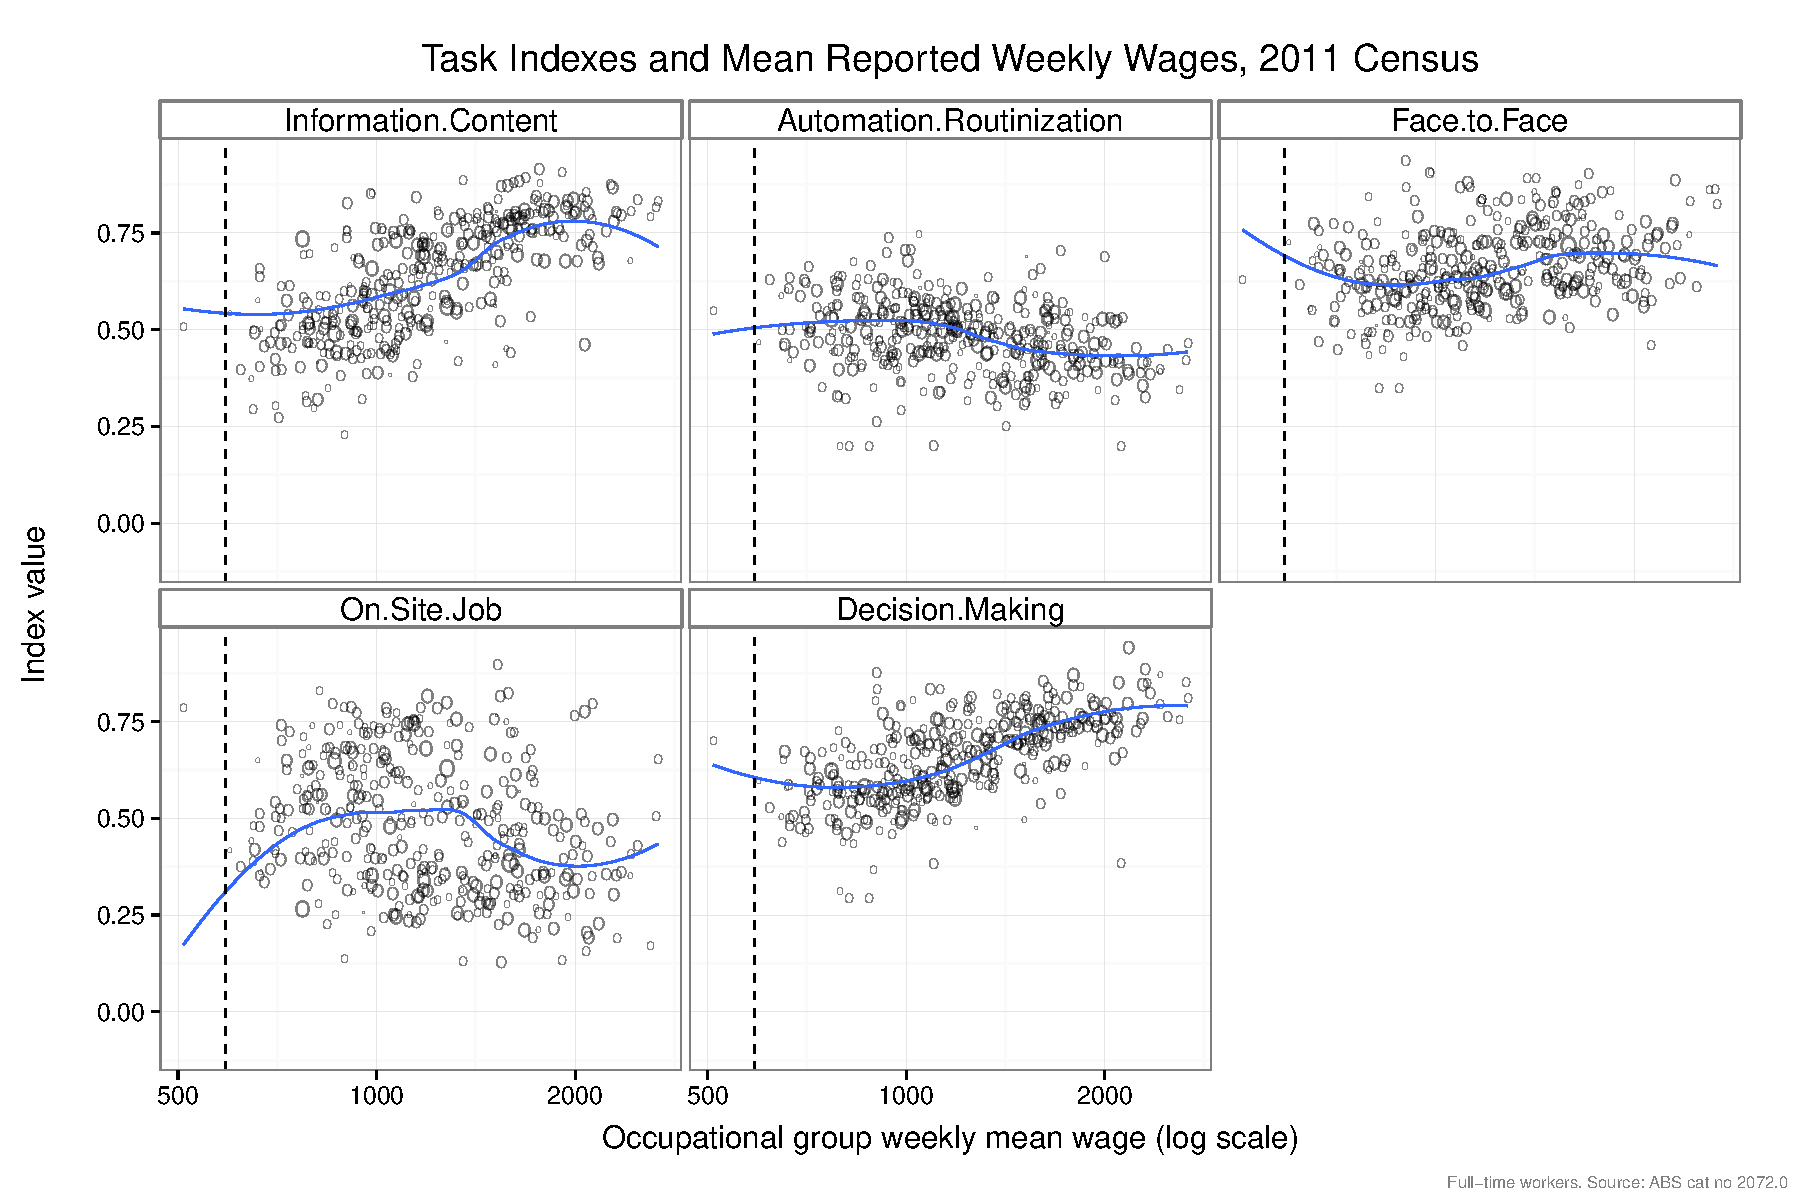
\includegraphics[width=\textwidth]{../figure/wages_indexes_4digit.pdf}
  \caption{Mean occupational weekly wage and task measure index values, at ANZSCO unit group (4-digit) level. The vertical dashed line is drawn at the level of the National Minimum Wage, of \$589.30 per week. Census respondents reporting full-time work are shown. The loess regression line is weighted by population; circle areas are proportional to population for each occupation. Notice that, when occupations are reduced to combined groupings, almost identical trends are observed (c.f. Figure~\ref{fig:meanocc2}). Sources: ABS cat 2072.0, O*NET, US Dept of Labor.}
  \label{fig:meanocc4dig}
\end{figure}
\documentclass{article}

\begin{document}

% Table created by stargazer v.4.5.1 by Marek Hlavac, Harvard University. E-mail: hlavac at fas.harvard.edu
% Date and time: Thu, Oct 10, 2013 - 12:36:34
\begin{table}[!htbp] \centering 
  \caption{Intercept and Slope of Change in Wage Quantiles, 1981/2 - 2011/12} 
  \label{} 
\begin{tabular}{@{\extracolsep{5pt}}lcccccc} 
\\[-1.8ex]\hline 
\hline \\[-1.8ex] 
 & \multicolumn{6}{c}{\textit{Dependent variable:}} \\ 
\cline{2-7} 
\\[-1.8ex] & \multicolumn{3}{c}{A (intercepts)} & \multicolumn{3}{c}{B (slopes)} \\ 
\\[-1.8ex] & (1) & (2) & (3) & (4) & (5) & (6)\\ 
\hline \\[-1.8ex] 
 Information.Content & 3.31 & $-$0.73 &  & $-$1.11 & 0.97 &  \\ 
  & (2.09) & (1.56) &  & (0.92) & (0.72) &  \\ 
  & & & & & & \\ 
 Automation.Routinization & $-$6.06 &  & $-$9.38$^{***}$ & 3.11$^{*}$ &  & 5.12$^{***}$ \\ 
  & (4.11) &  & (2.97) & (1.81) &  & (1.31) \\ 
  & & & & & & \\ 
 No.Face.to.Face & $-$0.01 & 1.39 &  & 0.26 & $-$0.48 &  \\ 
  & (2.96) & (2.29) &  & (1.30) & (1.05) &  \\ 
  & & & & & & \\ 
 No.On.Site.Work & 0.66 & 3.09$^{**}$ &  & $-$0.48 & $-$1.74$^{***}$ &  \\ 
  & (1.36) & (1.12) &  & (0.60) & (0.51) &  \\ 
  & & & & & & \\ 
 No.Decision.Making & 7.23$^{**}$ &  & 5.14$^{**}$ & $-$3.73$^{***}$ &  & $-$3.13$^{***}$ \\ 
  & (2.70) &  & (1.96) & (1.19) &  & (0.86) \\ 
  & & & & & & \\ 
 Constant & $-$1.35 & $-$0.97 & 3.46$^{***}$ & 0.39 & 0.19 & $-$1.68$^{***}$ \\ 
  & (1.85) & (1.52) & (1.05) & (0.81) & (0.70) & (0.46) \\ 
  & & & & & & \\ 
\hline \\[-1.8ex] 
Observations & 28 & 28 & 28 & 28 & 28 & 28 \\ 
R$^{2}$ & 0.50 & 0.33 & 0.29 & 0.57 & 0.38 & 0.40 \\ 
Adjusted R$^{2}$ & 0.38 & 0.25 & 0.23 & 0.48 & 0.30 & 0.35 \\ 
Residual Std. Error & 394.00 (df = 22) & 434.54 (df = 24) & 439.21 (df = 25) & 173.29 (df = 22) & 199.84 (df = 24) & 193.06 (df = 25) \\ 
F Statistic & 4.33$^{***}$ (df = 5; 22) & 3.96$^{**}$ (df = 3; 24) & 5.07$^{**}$ (df = 2; 25) & 5.90$^{***}$ (df = 5; 22) & 4.91$^{***}$ (df = 3; 24) & 8.25$^{***}$ (df = 2; 25) \\ 
\hline 
\hline \\[-1.8ex] 
\textit{Note:}  & \multicolumn{6}{r}{$^{*}$p$<$0.1; $^{**}$p$<$0.05; $^{***}$p$<$0.01} \\ 
 & \multicolumn{6}{r}{Occupational grouping #1 used, with 28 occupational groups.} \\ 
\normalsize 
\end{tabular} 
\end{table} 
\end{document}




% Table created by stargazer v.4.5.1 by Marek Hlavac, Harvard University. E-mail: hlavac at fas.harvard.edu
% Date and time: Fri, Oct 11, 2013 - 23:16:58
\begin{sidewaystable}[!htbp] \centering 
  \caption{Intercept and Slope of Change in Wage Quantiles, 2000/01 - 2011/12} 
  \label{} 
\begin{tabular}{@{\extracolsep{0pt}}lcccccc} 
\\[-1.8ex]\hline 
\hline \\[-1.8ex] 
 & \multicolumn{6}{c}{\textit{Dependent variable:}} \\ 
\cline{2-7} 
\\[-1.8ex] & \multicolumn{3}{c}{A (intercepts)} & \multicolumn{3}{c}{B (slopes)} \\ 
\\[-1.8ex] & (1) & (2) & (3) & (4) & (5) & (6)\\ 
\hline \\[-1.8ex] 
 Information content & $-$6.20 & $-$8.77$^{***}$ &  & 0.97 & 1.48$^{***}$ &  \\ 
  & (4.07) & (3.11) &  & (0.60) & (0.46) &  \\ 
  & & & & & & \\ 
 Automation/routinization & $-$8.22 &  & $-$17.16$^{***}$ & 1.14 &  & 2.58$^{***}$ \\ 
  & (8.60) &  & (6.04) & (1.27) &  & (0.89) \\ 
  & & & & & & \\ 
 No face-to-face contact & 3.72 & 2.33 &  & $-$0.41 & $-$0.41 &  \\ 
  & (6.14) & (4.00) &  & (0.90) & (0.60) &  \\ 
  & & & & & & \\ 
 No on-site work & 7.14$^{**}$ & 8.87$^{***}$ &  & $-$1.06$^{**}$ & $-$1.38$^{***}$ &  \\ 
  & (2.58) & (2.03) &  & (0.38) & (0.30) &  \\ 
  & & & & & & \\ 
 No decision-making & 5.39 &  & 12.92$^{***}$ & $-$1.02 &  & $-$2.16$^{***}$ \\ 
  & (5.05) &  & (4.09) & (0.74) &  & (0.60) \\ 
  & & & & & & \\ 
\hline \\[-1.8ex] 
Observations & 29 & 29 & 29 & 29 & 29 & 29 \\ 
R$^{2}$ & 0.48 & 0.44 & 0.29 & 0.51 & 0.47 & 0.34 \\ 
Adjusted R$^{2}$ & 0.36 & 0.38 & 0.24 & 0.40 & 0.40 & 0.29 \\ 
Residual Std. Error & 15.43 (23) & 15.23 (25) & 16.85 (26) & 2.27 (23) & 2.27 (25) & 2.48 (26) \\ 
F Statistic & 4.18$^{***}$ (5; 23) & 6.67$^{***}$ (3; 25) & 5.40$^{**}$ (2; 26) & 4.73$^{***}$ (5; 23) & 7.26$^{***}$ (3; 25) & 6.59$^{***}$ (2; 26) \\ 
\hline 
\hline \\[-1.8ex] 
\textit{Note:}  & \multicolumn{6}{r}{$^{*}$p$<$0.1; $^{**}$p$<$0.05; $^{***}$p$<$0.01} \\ 
 & \multicolumn{6}{r}{Occupational grouping 2 used, with 29 occupational groups.} \\ 
\normalsize 
\end{tabular} 
\end{sidewaystable} 



%%% Local Variables: 
%%% mode: latex
%%% TeX-master: "paper"
%%% End: 

\chapter{Conclusions \& Further Work}\label{ch:5}

\chapter{Conclusions \& Further Work}


\printbibliography

\appendix
\chapter{Data Construction}


\section{Survey of Income and Housing}

The Survey of Income and Housing (SIH) is a hierarchical, clustered sample survey of income and expenditure patterns of the the Australian population, periodically conducted by the Australian Bureau of Statistics. It was first conducted in the 1981-2 fiscal year, followed by 1985-6, and then every two or three years from 1994-5. Microdata files were obtained as confidentialized unit record files (CURFs) for the surveys performed in 1981-2, 1985-6, 1994-5, 1995-6, 1996-7, 1997-8, 2000-1, 2002-3, 2005-6, 2007-8 and 2009-10.

Unlike the Census, which is a population survey, the SIH is conducted on just a sample of the population, and unit records are weighted by demographic variables in order to create a representative sample. Weights are produced at three levels of the survey hierarchy: household, income unit and person. (In addition, the SIH is occasionally produced simultaneously with the Housing Expenditure Survey, or HES, in which case further expenditure levels are recorded.) For the purposes of this project, only individual-level records are of interest, and so results are weighted by person weight, $PERS\_WT$.

In all versions of the SIH, the $PERS\_WT$ variable for the $i$th record is computed as the reciprocal of that individual's probability of selection $\pi_i$:
$$ PERS\_WT_i = \frac{1}{\pi_i}, $$
$PERS\_WT_i$ can be interpreted as the number of individuals `represented' by record $i$. Note that the selection probabilities $\pi_i$, $i=1,\cdots,n$, need not sum to 1.

% repeated cross-section

\subsection{Data Processing Steps}

\section{Census}




%%% Local Variables: 
%%% mode: latex
%%% TeX-master: "paper"
%%% End: 

\chapter{Proof of Propositions in Chapter~3}

\newcommand{\ELL}{\mathcal{L}}
\newcommand{\EH}{\mathcal{H}}
\newcommand{\M}{\mathcal{M}}

First, suppose a competitive economy is governed by an CES aggregate production function which employs three types of workers: low-skilled, medium-skilled, and high-skilled. We do not necessarily require that workers of each type are homogeneous; but we do assume that the unit wage for each type of labor is fixed. 

Call the sets of high-, medium- and low-skilled workers $\EH$, $\M$, and $\ELL$, respectively. Then we can define the aggregate inputs of each worker type by summing over the inputs of each worker $i$, measured in efficiency units:
$$ H = \int_{i\in\EH}h_i\;di\quad 
     M = \int_{i\in\M}m_i\;di\quad
     L = \int_{i\in\ELL}\ell_i\;di $$

The aggregate production function also depends on ICT capital, $C$, which is a complement in production for high-skilled workers, and substitute for medium-skilled workers.
\begin{equation}\label{eq:prod}
Y =\left(\gamma  \left(C^{\eta }+H^{\eta }\right)^{\rho /\eta }+\beta  (C+M)^{\rho }+\alpha  L^{\rho }\right)^{1/\rho }
\end{equation}
For convenience, we'll assume the share parameters are equal and sum to unity, i.e. $\alpha=\beta=\gamma=1/3$.

Since the economy is competitive, the wage is given by each worker's marginal product, computed by taking the partial derivative of $Y$.
\begin{align*}
w_L &= \partial_LY \\
    &= \alpha  L^{\rho -1} \left(\gamma  \left(C^{\eta }+H^{\eta }\right)^{\rho /\eta }+\beta  (C+M)^{\rho }+\alpha  L^{\rho }\right)^{\frac{1}{\rho }-1} \\
w_M &= \partial_MY \\
    &= \beta  (C+M)^{\rho -1} \left(\gamma  \left(C^{\eta }+H^{\eta }\right)^{\rho /\eta }+\beta  (C+M)^{\rho }+\alpha  L^{\rho }\right)^{\frac{1}{\rho }-1} \\
w_H &= \partial_HY \\
    &= \gamma  H^{\eta -1} \left(C^{\eta }+H^{\eta }\right)^{\frac{\rho }{\eta }-1} \left(\gamma  \left(C^{\eta }+H^{\eta }\right)^{\rho /\eta }+\beta  (C+M)^{\rho }+\alpha  L^{\rho }\right)^{\frac{1}{\rho }-1}
\end{align*}

One way to achieve determinate comparative static predictions is to instead consider the {\em wage share}, computed as the wage bill for the labour type, divided by the total wage bill. These wage shares are:
\begin{align*}
\theta_H &= \frac{H w_H}{H w_H+L w_L+M w_M} \\
&= \frac{\gamma  (C+M) H^{\eta } \left(C^{\eta }+H^{\eta }\right)^{\frac{\rho }{\eta }-1}}{\alpha  (C+M) L^{\rho }+\beta  M (C+M)^{\rho }} \\
\theta_M &= \frac{M w_M}{H w_H+L w_L+M w_M} \\
&= \frac{\beta  M \left(C^{\eta }+H^{\eta }\right) (C+M)^{\rho -1}}{H^{\eta } \left(\gamma  \left(C^{\eta }+H^{\eta }\right)^{\rho /\eta }+\alpha  L^{\rho }\right)+\alpha  C^{\eta } L^{\rho }} \\
\theta_L &= \frac{L w_L}{H w_H+L w_L+M w_M} \\
&= \frac{\alpha  L^{\rho }}{\gamma  H^{\eta } \left(C^{\eta }+H^{\eta }\right)^{\frac{\rho }{\eta }-1}+\beta  M (C+M)^{\rho -1}}
\end{align*}
And the comparative statics are---
\begin{align*}
\frac{\partial \theta_H}{\partial C}
&= \frac{\gamma  H^{\eta } \left(C^{\eta }+H^{\eta }\right)^{\frac{\rho }{\eta }-2} \left(\beta  M (C+M)^{\rho } \left(C^{\eta } (C (-\eta )+C+M (\rho -\eta ))-C (\rho -1) H^{\eta }\right)-\alpha  C^{\eta } (C+M)^2 (\eta -\rho ) L^{\rho }\right)}{C \left(\alpha  (C+M) L^{\rho }+\beta  M (C+M)^{\rho }\right)^2} \\
&>0 \\
%
\frac{\partial \theta_M}{\partial C}
&= \frac{\beta  M (C+M)^{\rho -2} \left(\alpha  C (\rho -1) L^{\rho } \left(C^{\eta }+H^{\eta }\right)^2+\gamma  H^{\eta } \left(C^{\eta }+H^{\eta }\right)^{\rho /\eta } \left(C^{\eta } (C (\eta -1)+M (\eta -\rho ))+C (\rho -1) H^{\eta }\right)\right)}{C \left(H^{\eta } \left(\gamma  \left(C^{\eta }+H^{\eta }\right)^{\rho /\eta }+\alpha  L^{\rho }\right)+\alpha  C^{\eta } L^{\rho }\right)^2} \\
& < 0 \\
%
\frac{\partial \theta_L}{\partial C}
&= -\frac{\alpha  L^{\rho } \left(\beta  M (\rho -1) (C+M)^{\rho -2}-\gamma  C^{\eta -1} (\eta -\rho ) H^{\eta } \left(C^{\eta }+H^{\eta }\right)^{\frac{\rho }{\eta }-2}\right)}{\left(\gamma  H^{\eta } \left(C^{\eta }+H^{\eta }\right)^{\frac{\rho }{\eta }-1}+\beta  M (C+M)^{\rho -1}\right)^2} \\
& \gtrless 0
\end{align*}

%%% Local Variables: 
%%% mode: latex
%%% TeX-master: "paper"
%%% End: 

\end{document}

%%% Local Variables: 
%%% mode: latex
%%% TeX-master: t
%%% End: 
